\documentclass[main.tex]{subfiles}
\begin{document}
\glsresetall

\section{Introduction}

The first \gls{lst} was inaugurated in October 2018 and is currently taking its first data. It is the first \gls{cta} telescope installed on site (in La Palma island), and it is expected to be operating on its own until LST 2-4 are built. This mean that LST1 will need its own analysis chain in \textit{mono} mode, which differs in several aspects from the stereo analysis included in the benchmark analysis tools of \gls{cta} (see section \ref{sec:ctapipe}). Although single telescope observations present a big challenge, specially regarding source position reconstruction and $\gamma$-hadron separation, it is expected that LST1 performance, thanks to its size and camera design, will be competitive enough to offer scientific results in the time it will be operating alone.\\
This chapter will present a considerable amount of the work done during this thesis, which includes the development of the code for the single telescope analysis for LST1, the calculation of LST1 sensitivity based on \gls{mc} simulations, the development of a new technique for Hillas Parameters calculation without cleaning using the Expectation-Maximization algorithm and the application of the analysis chain to real LST1 data. 

\section{The LST1 analysis chain overview} \label{sec:anachain}

The software for the single telescope analysis of LST1, named \textit{cta-lstchain}, has been developed under the necessity of specific tools for single telescope analysis, which are not included in \textit{ctapipe}. It has been written as a python package which heavily relies on \textit{ctapipe}, and it is structured in several modules containing functions destined to the different parts of the analysis. The first version of \textit{cta-lstchain} was written by the author of this thesis and many contributors have joined the project over the last two years to improve and optimize the repository to its current version, which is able to perform every analysis step both for simulated \gls{mc} data and real data. The analysis chain is divided in several steps, each of which can be executed through a python script which requires certain inputs and calls for the appropriate functions. All the configuration parameters of the different elements of the analysis are given through configuration files, which can be edited by the user or else a standard configuration will be used. The input of the analysis chain are the raw data files of LST1 events, which for \gls{mc} data are the output files from \textit{sim$\_$telarray} (see section \ref{sec:simtel}), and for real data are \textit{zfits} files with a similar internal format. The files contain the full information available per pixel, known as \textit{waveform} and which is the digitized signal amplitude vs. time sample for every triggered event, together with \gls{mc} information in the case of a simulated file (such as the true energy, source position, number of simulated events, and so on), or recorded information from the different telescope subsystems in the case of real data (such as time, pointing, trigger type...). Throughout the analysis chain, the data including the images and image parameters, is stored in containers designed in \textit{cta-lstchain} specifically for LST1, which can be dumped into \textit{pandas} dataframes and saved in \textit{hdf5} files.\\
The main steps of the analysis chain can be summarized as: \\

\begin{itemize}
\item\textbf{Calibration:} The waveforms of each pixel in the camera should be integrated after pedestal subtraction, and converted to number of photoelectrons. Also, the timing information of the signal is obtained. 
\item\textbf{Image cleaning and parameterization:} The images in the camera contain pixels with light not related to the Cherenkov event, so a cleaning must be applied to remove them. Afterwards, the distribution of photons in the image is used to calculate the Hillas parameters.
\item\textbf{Energy and direction reconstruction:} The energy and direction reconstruction of the triggered events are performed using a multidimensional regression technique based on \glspl{rf}. A set of simulated diffuse $\gamma$ events are used to train the \gls{rf}. 
\item\textbf{$\gamma$-hadron separation:} For the $\gamma$-hadron separation, a multidimensional \gls{rf} classifier is used. Sets of simulated $\gamma$ and proton events, which energies and directions have been reconstructed in the previous step, are used to train the classifier.
\end{itemize}

\subsection{Calibration} \label{sec:calib}

In the calibration phase, the raw signal known as \textit{waveform} is integrated after background subtraction, to obtain a total number of counts per pixel, which afterwards is multiplied by a factor to be converted in number of photoelectrons. Depending on if \gls{mc} data or real data is being analyzed, the following steps vary and will be explained for each case.

\subsubsection{Signal extraction} \label{sec:signalext}

For every triggered event, the signal in each pixel is recorded in a 40 samples window from the 4096 samples of the \gls{dsr4}. This signal contains information not only from the Cherenkov light, but also from background light from \gls{nsb} and from the intrinsic noise induced by the readout chain. Before integrating the signal, it is necessary to subtract this baseline signal, known as \textit{pedestal}. For simulated \gls{mc} events the pedestal value for each pixel in the camera is already stored, but for real data it is necessary to take special pedestal runs, with randomly activated trigger. Pedestal events are used to calculate the mean pedestal value for each \gls{dsr4}, Typically, around 1000 events are needed to fill the ring. In \textit{cta-lstchain} a specific script is used to extract the pedestal values from pedestal runs and they are stored in a \textit{hdf5} file to be used later in the calibration.\\
Once the pedestal is subtracted from the signal, the signal peak can be integrated. Typically a smaller window of a few samples around the maximum is used for the integration, which can be performed with one of the several integrators implemented in \textit{ctapipe}. By default, the integrator used in \textit{cta-lstchain} is the \textit{NeighborPeakWindowSum}, which sums the signal in a window around the peak defined by the waveform in neighbouring pixels. This allow to avoid integrating peaks which can arise from fluctuations. The default width of the integration window for this integrator is of 7 samples, but it can be configure by the user. These calibration steps are performed for the two gain channels of \gls{lst}1 camera. 

\subsubsection{Conversion to photoelectrons}

Once the signal amplitude is extracted, it must be converted from DC counts to photoelectrons through a calibration factor, which is different for each pixel and channel. For simulated \gls{mc} data, these factors are stored in the simulated file and the conversion can be done simply by multiplying the image in DC counts by the factor of each pixel. For real data, special calibration runs must be taken to calculate these factors. Calibration events are taken using Ultraviolet light pulses fired from the CaliBox \cite{2015CaliBox}, \cite{2019CaliBox} located in the mirror dish. The calculation of the calibration coefficients is made using the F-factor method \cite{1997calibrationPMT}, which assumes that the distribution of photoelectrons in a \gls{pmt} follows a poissonian statistics with a mean $N$ and a \gls{rms} $\sqrt{N}$. The signal distribution, however, will be deviated from a poissonian statistics with a wider \gls{rms} due to an excess-noise factor F, which is different for each \gls{pmt} and is measured in the laboratory. The relation between the relative widths of the two distributions can be written as:

\begin{equation}
  F \cdot \frac{1}{\sqrt{N}} = \frac{\sigma_{Q}}{<Q>}
  \label{eq:ffactor}
\end{equation} 

Where $<Q>$ is the mean value of the pixel signal and $\sigma_{Q}$ its \gls{rms}. The calibration coefficients will come from the relation between the number of photoelectrons $N$ and the mean pixel signal $<Q>$. From \ref{eq:ffactor}, and taking into account that the signal must be corrected from pedestal, the relation between number of photoelectrons $N$ and the pixel charge $<Q>$ is:

\begin{equation}
  \frac{N}{<Q>} = F^{2}\frac{<Q> - <ped>}{\sigma_{Q}^{2} - \sigma_{ped}^{2}}
\end{equation}

The values of $<Q>$, $\sigma_{Q}$, $<ped>$ and $\sigma_{ped}$ are calculated from a sufficiently large number ($\sim$ 1000) of calibration and pedestal events, using a specific script from \textit{cta-lstchain}, which stores the resulting calibration coefficients in an \textit{hdf5} file to be used later in the calibration of data runs. For the LST1, the value of F factor used is the mean value for all \gls{pmt} which is 1.2.

\subsection{Image cleaning and parameterization} \label{sec:cleanpars}

In order to extract information from the image of Cherenkov light recorded by the camera, it is necessary to get rid of the background light not belonging to the event, which has arrived to all pixels. This background light is usually related to fluctuations in the \gls{nsb}. A process named cleaning is used to eliminate all pixels which presumably do not contain light from the shower. The \textit{clean} image is used later to perform the Hillas parameterization. Besides there exist several proposed cleaning algorithms in the literature \cite{2019cleaningCNN}, \cite{2013neighborcleaning}, \cite{2005Cleaningwithtimeinfo}, \cite{2001waveletcleaning}, for the time being in \textit{cta-lstchain}, a classical two-level tailcuts cleaning is being applied (like the one used in \cite{1997HEGRAperformance}). This method requires only the information of the amount of light in pixels (already converted to number of photoelectrons) and compares it to two levels of thresholds in the following way: \\

\begin{itemize}

\item Pixels with a number of photoelectrons over the highest threshold level $Th_{high}$ are selected.
\item If pixels selected in the previous step have at least one neighbour also above the highest level threshold, those pixels are marked as core pixels from the shower.

 \item Neighbours of the core pixels with number of photoelectrons above the lower level threshold $Th_{low}$ are selected as boundary pixels. For the rest of them not selected, their charge is set to zero. \\
\end{itemize}
   
   The standard values for the two levels used in \textit{cta-lstchain} are $Th_{high} = 6$ phes and $Th_{low} = 3$ phe. Note that these values have not been yet fully optimized for the particular case of the \gls{lst}1, and they can be changed easily in the configuration files. An optimization of the cleaning can lead to a better performance, specially for lower energies, because in those cases Cherenkov showers are small and a lot of information can be lost because of cleaning. Using other information apart from the number of photoelectrons, like the arrival times of the signals to pixels, can help to improve the image parameterization. Low energy showers of $\gamma$s and hadrons are much more difficult to differentiate, for that reason, an image parameterization which highly depends on the settings of the cleaning parameters can be problematic when trying to lower the energy threshold of the telescope. In section \ref{sec:EM} a method for image parameterization not requiring previous cleaning is proposed as an alternative.\\
   The parameterization of the shower image after cleaning, meaning the calculation of the Hillas parameters (see section \ref{sec:IACTs} and figure \ref{fig:hillas}), is performed by a specific function from \textit{ctapipe}. The resulting parameters: intensity (total number of photoelectrons in the shower), width, length, coordinates of ellipse center of gravity, azimuthal angle $\phi$, the orientation angle $\psi$, and the third order moments: \textit{skewness}, which is a measure of the asymmetry of the distribution; and \textit{kurtosis}, which is a measure of whether the distribution is peaked or flat relative to a normal distribution. The calculation of the Hillas parameters with \textit{ctapipe} only requires the image of the shower (i.e. the number of photoelectrons in each pixel) and the information of the camera geometry.\\
   The time parameters, \textit{time gradient} and \textit{intercept} are also calculated as explained in section \ref{sec:ctapipe}. These two parameters are specially important for single telescope analysis, because they reflect the direction of development of the shower, which give information of the side of the ellipse where the source position is located in the camera frame.\\
   Other parameters are the \textit{leakage2}, which indicates the percentage of the shower that falls in the two outer pixel rings of the camera. A large leakage indicates that the shower is highly truncated. The \textit{number of islands} is also calculated, which accounts for the number of separated groups of pixels in the image. A typical $\gamma$-ray shower will only have one island with elliptical form, but hadronic and heavier nuclei showers tend to produce messy light distributions with several islands of irregular shapes.\\
   
The calibration and image parameterization is performed in \textit{cta-lstchain} using the scripts \textit{$lstchain\_data\_r0\_to\_dl1.py$}, \textit{$lstchain\_mc\_r0\_to\_dl1.py$}, depending on if the raw data used is simulated or real data. As is reflected in the script names, this steps reduces the data level from raw R0 data to DL1 (see table \ref{tab:CTAdatalevels}). In general, the image parameters can well describe the shower and therefore pixel wise information is not needed in further steps of the analysis. However, for testing and crosscheck purposes, \textit{cta-lstchain} scripts offer the possibility to store DL1 data with the full images.


\subsection{Reconstruction of energy and source position} \label{sec:recoe}

After the calibration and image parameterization, the image parameters should be used to extract information of the primary particle, whereas is a $\gamma$-ray or a background event (protons, electrons, heavier nuclei...). In \textit{cta-lstchain} the first step is to reconstruct the energy and arrival direction of the event.\\ 
The direction reconstruction is problematic in single telescope mode, because even knowing that the Hillas ellipse should point towards the source position in the camera frame, we do not know in which side of the ellipse is located (this is known as head-tail degeneracy). In stereo mode, this is solved because the source position will be in the cross point between the line which follows the semi major axis of Hillas ellipses of all cameras, but for single telescope we must rely in other methods. In the case of \textit{cta-lstchain} we make use of a vector known as \textit{disp}. This is the vector going from the center of gravity of the ellipse to the source position.\\
Originally, the disp quantity could be parameterized in terms of the elongation of the image, meaning the ratio between \textit{width} and \textit{length}. The first parameterization was proposed by the Whipple collaboration \cite{1994dispwhipple}:

\begin{equation}
  Disp = \xi \cdot \left(1 - \frac{width}{length}  \right)
\end{equation}

Where $\xi$ is a factor dependent on the amount of photoelectrons in the shower image (the \textit{intensity} parameter). A more general parameterization was used for MAGIC-I \cite{2005DISPmagic}:

\begin{equation}
 Disp=A(intensity) + B(intensity) \cdot \frac{width}{length+\rho(intensity) \cdot leakage}  
\end{equation}

Where A, B and $\rho$ are the second order polynomial function parameters of log(\textit{intensity}).\\

Instead of using a parameterization, in \textit{cta-lstchain} the disp vector is directly reconstructed using the image parameters. The time parameters will be very important to reconstruct this quantity, because the Cherenkov light from the upper parts of the shower arrive before the light from later developed lower parts, giving the time gradient. The time gradient will therefore give information on which side of the ellipse is pointing to the source position.\\

The method used in \textit{cta-lstchain} for the reconstruction of these quantities, energy and disp vector, is based on a multidimensional regression technique relying on \glspl{rf}. \gls{rf} is a supervised learning algorithm which uses an ensemble of several decision trees (this is known as a \textit{bagging} technique). Decision trees are flow-chart-like structures where each internal node denotes a test on a selected feature. The result is a split in the dataset depending on the value of that feature. The best splitting criterion for regression is typically calculated using the \gls{mse}. For each node, the \gls{mse} of the two subsets is calculated for each feature and for each possible cut on that feature, until a minimum is reached. This step is repeated at each node until a condition is reached, typically that the \gls{mse} of the remaining data sample is below a threshold, or it has too few events to keep splitting. The termination nodes are also known as \textit{leaves}.
In the \gls{rf}, a number of decision trees are trained using a randomly selected subset of the train data (\textit{'bootstrapping'}) and the prediction of all the trees is averaged to reach the final result. Also, the features are always randomly permuted at each split. These two sources of randomness in the \gls{rf} prevent the typical problem of over-fitting from too complicated decision trees. 

In the basic analysis of \textit{cta-lstchain}, the one carried on in this thesis, a source independent approach is used, where it is not assumed what is the true position of the source. For that reason, the \glspl{rf} for energy and disp reconstruction are trained using a set of \gls{mc} simulated $\gamma$ events triggering the \gls{lst}1, with diffuse arrival directions distributed in a 5º radius \gls{fov}. The set of simulated data is divided in two sets, for training and testing. The features used for the splitting of the tree nodes are $log_{10}(intensity)$, \textit{width, length, x, y, psi, phi, width/length, skewness, kurtosis, r, time gradient, intercept, leakage} and \textit{number of islands}, where x, y and r are the coordinates and module of the vector from center of gravity of the Hillas ellipse to the center of the camera. These features can be ordered based on their importance for the regression, as shown in figure \ref{fig:importances}. It can be seen for example that for direction reconstruction there are two features, time gradient and angle $\psi$, which are the best candidates to make a good splitting, while for $\gamma$-hadron separation all features supply with a similar amount of information. 
The trained \glspl{rf} are used later to reconstruct the desired values (energy and disp) in the test data. For energy reconstruction, the reconstructed quantity is actually $\log_{10}(E)$. In the case of the disp vector, the two components of the vector (\textit{disp\_dx, disp\_dy}) are reconstructed using the same \gls{rf}.\\
For the implementation of the \glspl{rf}, the Python package \textit{scikit-learn} \cite{2011scikit-learn} is used, a machine learning package which offers a large amount of tools for predictive data analysis. The class \textit{RandomForestRegressor} allow an easy training of the \glspl{rf}, which can be saved to be used later to fit any set of test data with the same format as the training set. This class has a set of parameters that can be modified by the user to optimize the performance of the predictions. In \textit{cta-lstchain} these parameters can be modified by a configuration file. The most relevant parameters and their default values in \textit{cta-lstchain} are shown in table \ref{tab:RFpars}. 

\begin{table}
  \centering
  \begin{tabular}{|l|l|l|l|}
    \hline
    Parameter name & Value          & Value              & Description\\
                   & for regression & for classification &  \\ 
    \hline
    n\_estimators       & 150 & 100  & \small{Number of trees in the forest}\\
    criterion           & mse & gini & \small{Function to measure the quality of a split}\\
    max\_depth          & 50  & 100  & \small{Maximum depth of the tree}\\
    min\_samples\_split & 2   & 2    & \small{Minimum number of samples required to}\\
                        &     &      & \small{split an internal node} \\ 
    min\_samples\_leaf  & 2   & 2    & \small{Minimum number of samples to be at a}\\
                        &     &      & \small{leaf node} \\     
    max\_features       & all & all  & \small{Number of features to consider when looking} \\
                        &     &      & \small{for the best split}\\
    random\_state       & 42  & 42   & \small{Control the randomness of the} \\
                        &     &      & \small{bootstrapping and the sampling of features}\\
    n\_jobs             & 4   & 4    & \small{Number of jobs to run in parallel}\\
    \hline
  \end{tabular}
  \caption{Some parameters that can be configured for \textit{RandomForestRegressor} and \textit{RandomForestClassifier} classes, with the default values used in \textit{cta-lstchain}.}
  \label{tab:RFpars}
  \end{table}

\begin{figure}
\centering
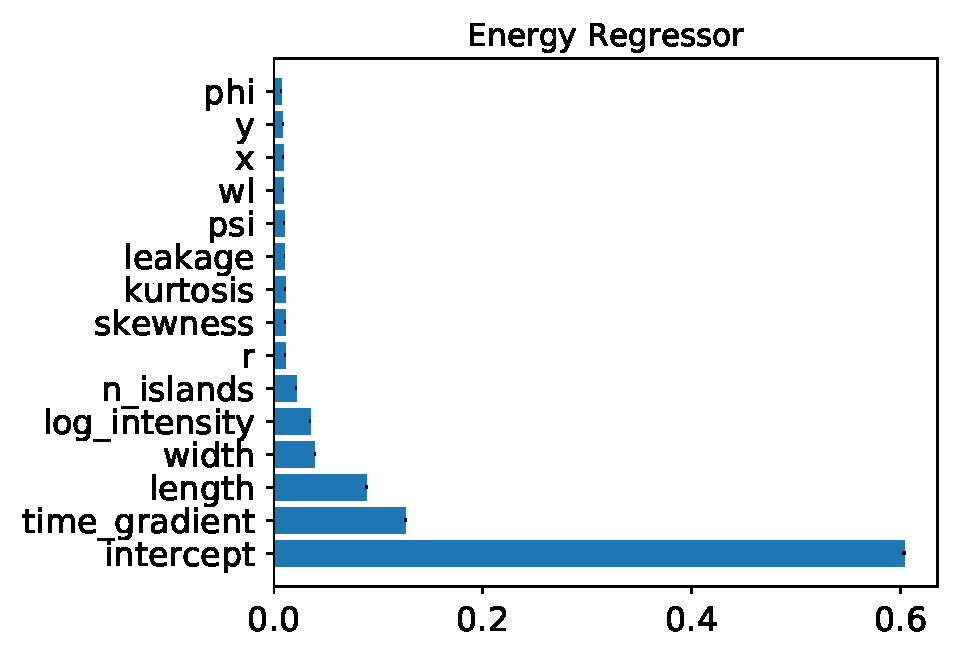
\includegraphics[width=0.45\textwidth]{Pictures/reg_energy_importances.pdf}
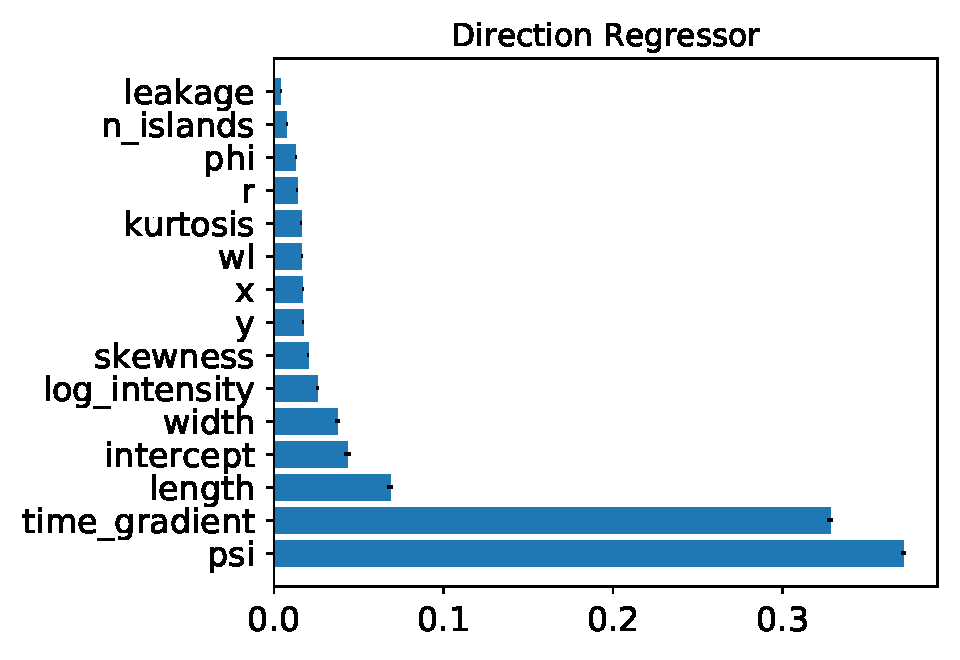
\includegraphics[width=0.45\textwidth]{Pictures/reg_disp_vector_importances.pdf}
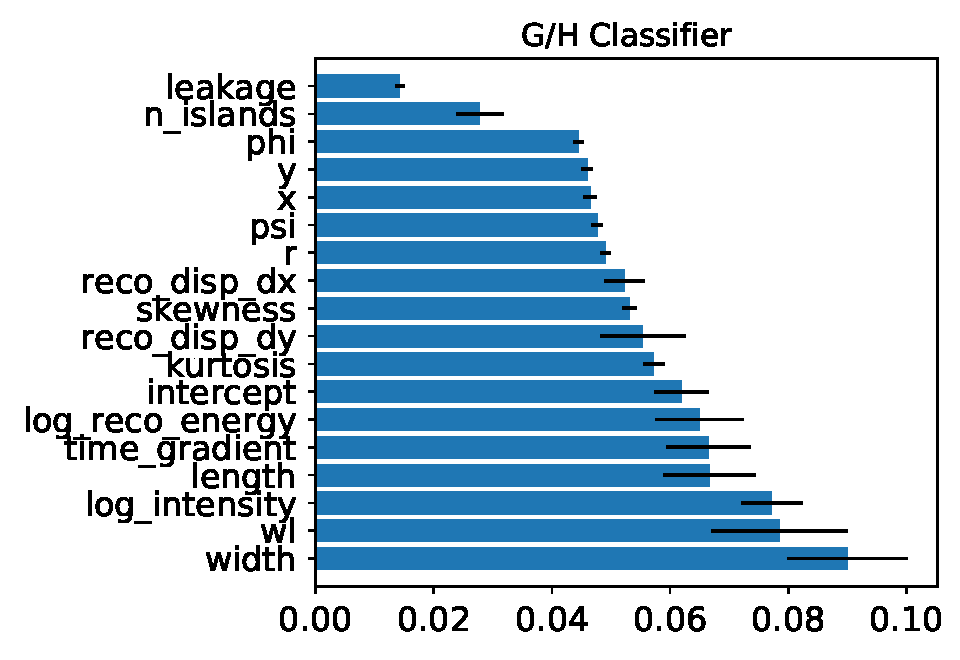
\includegraphics[width=0.45\textwidth]{Pictures/gls_importances.pdf}
  \caption{Feature importances for the trained \gls{rf} used in the analysis of \gls{mc} simulated \gls{lst}1 data. The higher the importance value, the more relevant is the feature for the regression/classification. }
    \label{fig:importances}
\end{figure}


\subsection{$\gamma$-hadron separation} \label{sec:gammahsep}

The majority of Cherenkov showers produced in the atmosphere are actually not produced by $\gamma$-rays, but by cosmic hadrons (mainly protons). These events trigger the telescopes $\sim 10^4$ times more than $\gamma$-rays, therefore it is necessary a very efficient background rejection method to discard hadronic showers and analyze only $\gamma$ events. The methods for $\gamma$-hadron separation in general rely on the morphological differences between the showers produced by the two kinds of particles, including temporal information. This job is much more efficient in stereo mode, because $\gamma$-ray showers which trigger different telescopes will produce images in the cameras with a Hillas ellipse pointing towards the source position, while hadronic showers will produce much less correlated images. In mono mode we can only rely on the morphological features of the images, knowing that hadronic shower images will be much more extended, without a clear definite shape and with a higher number of islands than $\gamma$ showers.\\
The task of $\gamma$-hadron separation is done in \textit{cta-lstchain} with a \gls{rf} classifier, which follows similar principles as the \gls{rf} regressor explained in the previous section. Instead of calculating the value of a variable, it decides between a given number of classes to which each events belongs. In this case, its only a two classes problem: $\gamma$s or hadrons.
The best splitting criterion for classification is calculated in terms of the so-called gini index. The gini index o gini impurity is a measure of how often a randomly chosen event would be incorrectly classified if it was classified randomly following the distribution of classes. The formula for the Gini index $I_G$ calculated for a set of events with J classes is:

\begin{equation}
  I_G(p) = 1 - \sum_{i=1}^J p_i^2
\end{equation}

Where $p_i$ is the probability of an event belonging to the class $i$ to be correctly classified.  The Gini index go from 0 to 1, where 0 means that all the events of a subset have been classified to one class, and 1 that the events of the subset are randomly distributed along all the possible classes. The splitting decision will be made minimizing the value of the Gini index.\\
The training set for the $\gamma$-hadron classifier will consist on two sets of \gls{mc} simulated events, one of diffuse $\gamma$s and one of protons, with arrival directions coming from a 10º radius \gls{fov}. Usually, the set of hadronic events used for training is taken from real background events recorded with the telescope when pointing to a direction in the sky without any $\gamma$-ray source, because the simulation of proton showers has a lot of uncertainties (see section \ref{sec:corsika}). However, as by the time this thesis was written there were not enough real data from \gls{lst}1 to build a big enough background data set, all the calculations have been made using \gls{mc} simulations.\\
The features used for the splitting of the classifiers are the same from the ones used for the regressors of the previous section, but adding the reconstructed energies and disp vector. To do so, the original $\gamma$ events set is splitted in a training set for the regressor, and a test set, to which the energy and disp vector are reconstructed. The regressors are also used to reconstruct the energy and disp vector of the set of proton events. Afterwards, this new set of $\gamma$ and proton events, with reconstructed energy and disp is divided again in a training and test set to build the \gls{rf} classifier.
The classifier is implemented using the \textit{RandomForestClassifier} class from \textit{scikit-learn} which input parameters are listed in table \ref{tab:RFpars}


\section{Sensitivity of the LST1}

The sensitivity of a telescope is defined as the minimum flux of $\gamma$-rays over background that should be detected for a statistically significant detection. Using the simulated \gls{mc} data and the analysis techniques explained in section \ref{sec:anachain} the differential sensitivity of \gls{lst}1 in mono mode can be calculated.\\
The sensitivity is computed for the detection of a point source after 50 hours of observations. To do so, we are using the Li\&Ma method, extensively described in \cite{1983LiMa}, but here the basic concept is summarized.\\
The significance of detection of a source must be calculated, as a way to evaluate the statistical reliability of an observational result. A typical observation in $\gamma$-ray astronomy will consist on pointing to a region where it is suppose to exists a source, recording $N_{on}$ counts in a time $t_{on}$. Then, to evaluate the background, a region without any source is observed, recording $N_{off}$ counts in a time $t_{off}$. If the ratio between the observation time of the on and off regions is $\alpha = t_{on}/t_{off}$ then the number of background photons in the on region is estimated by $\hat{N}_{B} = \alpha N_{off}$  and the probable number of photons contributed by the source is $N_{S} = N_{on}-\alpha N_{off}$. The significance can be estimated in terms of the likelihood ratio method, where the we test the \textit{null hypothesis}, being the hypothesis where no source exist at all and all the excess counts detected in the on region are due to fluctuations in the background. In this case, $N_{on}$ will follow a Poisson distribution with variance equal to that of the background $<N_{B}>$. The likelihood ratio can be written as:

\begin{equation}
  \lambda = \frac{L(X | E_{0}, \hat{T}_{c})}{L(X|\hat{E},\hat{T})}
\end{equation}

Where X are the observed data and (\^{E},\^{T}) are the maximum likelihood estimation of the unknown parameters. In the null hypotheses, $E=E_{0}$ and $T=\hat{T}_{c}$ are the parameters for the conditional maximum likelihood estimation. In our case, the unknown parameters will be $N_{S}$, $N_{B}$ where in the null hypothesis $N_{S}=0$.\\
The maximum likelihood ratio has the form:

\begin{equation}
  \lambda = \left[ \frac{\alpha}{1+\alpha}\left( \frac{N_{on}+N_{off}}{N_{on}}\right) \right]^{N_{on}} \left[ \frac{1}{1+\alpha}\left( \frac{N_{on}+N_{off}}{N_{off}}\right)\right]^{N_{off}}
\end{equation}

If the null hypothesis is true, and $N_{on}, N_{off} \gtrsim 10$, by the theorem exposed in \cite{1983LiMa}, the quantity $-2ln\lambda$ will asymptotically follow a $\chi^2$ distribution with one degree of freedom. Therefore $\sqrt{(-2ln\lambda)}$ will be equivalent to the absolute value of a standard normal variable, so we can take it as the significance:

\begin{equation}
  S = \sqrt{(-2ln\lambda)}
\end{equation}

Typically, a detection is claimed when the significance $S$ is equal to or higher than 5 ($5\sigma$ detection). To calculate the sensitivity of \gls{lst}1 we need to know the number of excess counts from a hypothetical source $N_{S}$ that will lead to $S=5$ for $\alpha=1/5$. \\
To perform this calculation, we need to estimate the number of background (proton) events ($N_{B} = \alpha N_{off}$) that will remain after analyzing the data and doing the $\gamma$-hadron separation. The steps followed to do so are described in the next sections.

\subsection{Reweigh ting}

The \gls{mc} simulations of \gls{eas} used for this work were simulated as if the particles ($\gamma$s or protons) followed a power law spectrum
:
\begin{equation} \label{eq:powerlaw}
\frac{dN}{dE} = K E^{a}
\end{equation}

with a spectral index $a=-2$. However, we want to give the sensitivity with respect to the true spectrum of protons, and typically, the spectrum of the Crab nebula is used for the $\gamma$-rays. We need to transform the distribution of simulated events from number of events per energy to a rate of events (events per unit time) per energy which follow the desired spectral shape. We will calculate a spectral weight $w(E)$ for each event, which will depend on its true energy.\\
Suppose that $N$ \gls{mc} events have been generated in the energy range $(E_1,E_2)$, following the power law from \ref{eq:powerlaw}, with isotropically distributed directions in a solid angle $\Omega$ and impact parameters uniformly distributed in a circular area A, orthogonal to the incident direction of the particles.
The quantity $K$ will be:

\begin{equation}
  K = \frac{N(a+1)}{E_{2}^{a+1}-E_{1}^{a+1}}
\end{equation}

We want to change the shape of this spectrum, and get a new differential spectrum of the shape:

\begin{equation}
  \frac{dF}{dE(E)} = \frac{dF}{dE(E_0)}\cdot f(E/E_0)
\end{equation}

Where $\frac{dF}{dE(E_0)}$ is a normalization factor referring to an arbitrary energy $E_0$, which should be between $E_{1}$ and $E_{2}$, with units $s^{-1}sr^{-1}m^{-2}TeV^{-1}$ and f is a function that satisfies $f(E=E_{0}) = 1$. In our case, f will simply be the new power law. To correct the $dN/dE$  simulated spectrum to the desired power law, we should multiply it by $(E/E_{0})^{-a}$, so it will become flat, and then by $f(E/E_{0})$ to get the correct form. Weighting by these two factors, the corrected number of \gls{mc} events $N'$ will be the integral:

\begin{equation}
  N' = \int^{E_{2}}_{E_{1}} \left(\frac{E}{E_{0}}\right)^{-a} f(E/E_{0}) dE = \int^{E_{2}}_{E_{1}} KE_{0}^{a}f(E/E_{0})dE
\end{equation}

We need to transform the number of events to a rate (in Hz), in order to calculate the sensitivity for a certain observation time. The total rate calculated in the energy range $E_{1}, E_{2}$ will be:

\begin{equation}
  R = \int^{E_{1}}_{E_{2}} \frac{dF}{dE}dE d\Omega dA
\end{equation}

Therefore, the final weight $w(E)$ for which the spectrum of each event should me multiplied is:

\begin{equation}
  w(E) = \left(\frac{E}{E_0}\right)^{-a}\cdot f(E/E_{0}) \cdot \frac{N'}{R}
\end{equation}

Where $a=-2$ is the spectral index of the simulated events, $E_{0}$ is taken as 1 TeV and $f(E/E_{0})$ would depend on the spectral shape to be reproduced. For $\gamma$ events we take the spectrum of the Crab nebula measure by HEGRA \cite{2004CrabHEGRA}:

\begin{equation}
  \left(\frac{dF}{dE}\right)_{Crab} = 2.83\cdot 10^{-14} \left(\frac{E}{1 TeV}\right)^{-2.62} GeV^{-1}cm^{-2}s^{-1}
\end{equation}

And for protons, we use the results from the BESS spectrometer \cite{2000protonBESS}:

\begin{equation}
    \left(\frac{dF}{dE}\right)_{Crab} = 9.6\cdot 10^{-9} \left(\frac{E}{1 TeV}\right)^{-2.7} GeV^{-1}cm^{-2}s^{-1}
\end{equation}

The values of the differential sensitivity will be given for a certain number of energy bins, therefore, we must calculate the number of weighted events in each energy bin and multiply them by the observation time. This will give us the quantities $N_{S}$ and $N_{B}$. To calculate the sensitivity we only need $N_{B}$, which will be the number of weighted proton events divided by the factor $\alpha = 1/5$.

\subsection{Cut optimization}

To obtain the best possible sensitivity, instead of using all the weighted proton events, we can use the two parameters $gammaness$ and $\theta^2$ to perform cuts that will reject the majority of the background.\\
$Gammaness$ is a number between 0 and 1 assigned by the \gls{rf} classifier to make the decision on the $\gamma$-hadron separation. Events close to 1 will be more $\gamma$-like, and events close to 0 will be more proton-like.
$\theta^2$ is the angle between the reconstructed direction of the event and the true assumed direction of the source. Events with a high $\theta^2$ are most likely to be proton events, while $\gamma$s will have a $\theta^2$ close to 0. For protons, 
\\
To optimize the cuts in these parameters, we define several bins in $gammaness$ and $\theta^2$, calculate the number of weighted proton events left after the cuts in each bin and then use this quantity as $N_{B}$ for the sensitivity calculation. For each energy bin, we will select the combination of cuts which provides the best sensitivity. We require that after the cuts, at least 10 events of $\gamma$s and protons remain in the energy bin.  

\subsection{Expected LST1 Performance}\label{sec:performance}

The analysis methods described before were used to compute the expected performance of the LST1 in mono mode for the observation of a point source, using a source independent analysis (meaning no assumption on the source position is made). In this section, the results on energy and angular resolution, $\gamma$-hadron separation and sensitivity are discussed.

\subsubsection{Data} \label{sec:mcdata}

The data used for the analysis is a set of \gls{mc} simulations produced specifically for the \gls{lst}1 in the northern \gls{cta} site. The primaries produced were $\gamma$s as a point source with an offset of 0.4º from the center of the camera, diffuse $\gamma$s, protons and electrons, but for the results given in this thesis, electrons were not included. The injection of particles were splitted in North and South, but only the South production has been used here. The zenith angle assumed was 20º, the spectral index of the particle spectra was -2. A summary of the main features of the production is given in table \ref{tab:mcprod}.

\begin{table}
  \centering
    \begin{tabular}{|l|l|l|l|l|}
      \hline
      & $\gamma$ (PS) & $\gamma$ diffuse & electron & proton\\
       & offset = 0.4º & & & \\
      \hline
      Energy Range & 5 GeV - 50 TeV & 5 GeV - 50 TeV & 5 GeV - 5 TeV & 10 GeV - 100 TeV\\
      Viewcone     & 0 º  & 10º & 10º & 15 º \\
      Core Range  & 1000 m & 1000 & 1000 m & 2500 \\
      Input Events & South: $3\cdot 10^7$ & South: $5\cdot 10^8$ & South: $6\cdot 10^8$ & South: $5\cdot 10^9$ \\
      & North: $3\cdot 10^7$ & North: $5\cdot 10^8$ & North: $6\cdot 10^8$ & North: $5\cdot 10^9$ \\
      Triggered Events & South: $1.08\cdot 10^6 $ & South: $1.22\cdot 10^6 $ & South: $1.18\cdot 10^6 $ & South: $8.25\cdot 10^5 $ \\
      & South: $9.60\cdot 10^5 $ & South: $1.11\cdot 10^6 $ & South: $1.04\cdot 10^6 $ & South: $8.10\cdot 10^5 $ \\
      \hline
      \end{tabular}
  \caption{Summary of the \gls{mc} production dedicated to the \gls{lst}1}\label{tab:mcprod}
\end{table}

After calibrating and parameterizing the data, using three sets of cleaning parameters to study the effect on cleaning in the analysis, the diffuse $\gamma$ events were used to train the \gls{rf} regressors. Then, a subset of diffuse $\gamma$s and the hadron events to which the energy and direction was reconstructed, were used to train the \gls{rf} classifier for $\gamma$-hadron separation.
The point source $\gamma$s, together with a subset of hadron events as background, have been used to produce the performance results. A filter in intensity > 300 phe, leakage < 0.2 and gammaness > 0.5 was applied to the reconstructed events.  

\subsubsection{Energy resolution}

The energy resolution give information on the error committed while reconstructing the energy of an event. It is defined as the 68th percentile of the relative error $\Delta E/E = (E_{reco}-E_{true})/E_{true}$. If the relative error follows a normal distribution, the 68th percentile is equivalent to one $\sigma$. The results on energy resolution are shown in figure \ref{fig:energy}. The features used for the energy regression ordered by their importance can be sen in figure \ref{fig:importances}.

\begin{figure}
\centering
 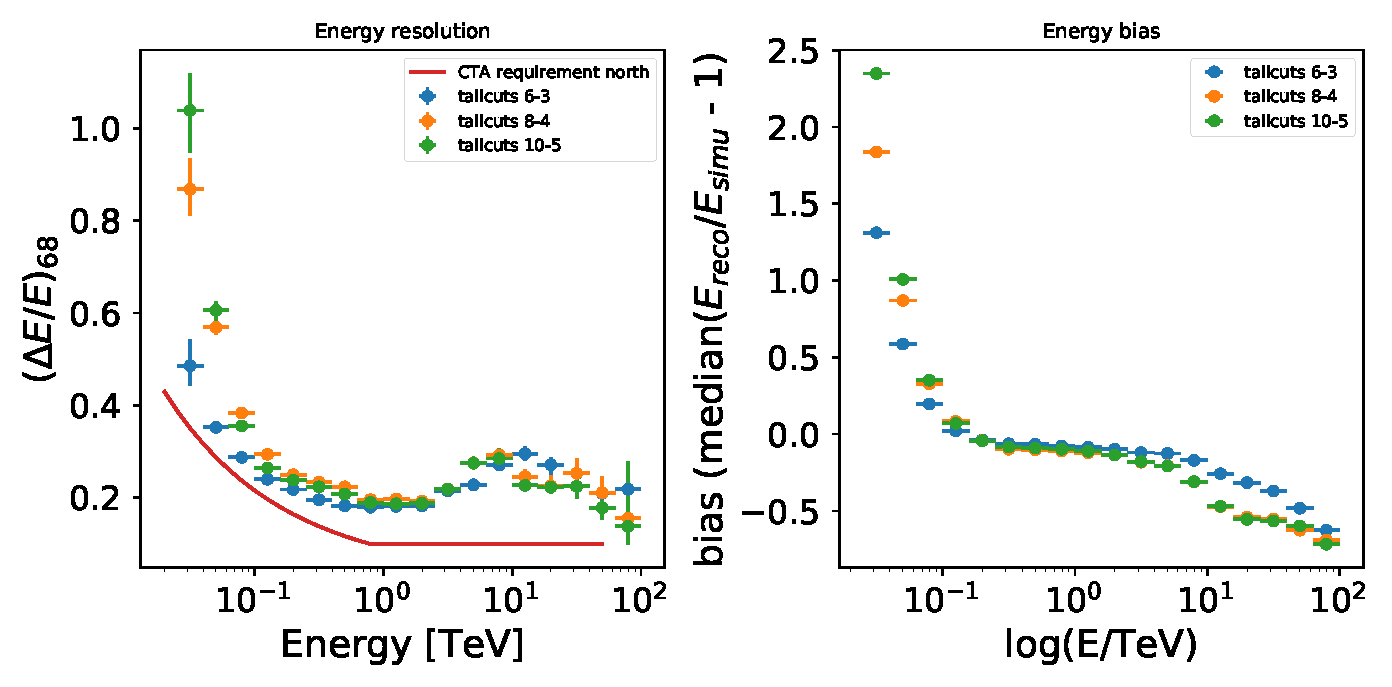
\includegraphics[width=1\textwidth]{Pictures/energy_resolution.pdf}
  \caption{Energy resolution plots for the \gls{lst}1 analysis applied to a \gls{mc} production of point-like $\gamma$ events, for three different sets of cleaning parameters (low level-high level threshold in number of photoelectrons). As a reference, the energy resolution requirement for \gls{cta}-north is also shown. The energy resolution plot of the \textit{left} has been bias corrected.}
    \label{fig:energy}
\end{figure}



\subsubsection{Angular resolution}

The angular resolution is calculated in a similar way as the energy resolution, but in this case the relative error shown in figure \ref{fig:angres} refers to the angular difference between the true direction of the source and the reconstructed direction. The features used for the disp vector regression ordered by their importance can be sen in figure \ref{fig:importances}.


\begin{figure}
\centering
 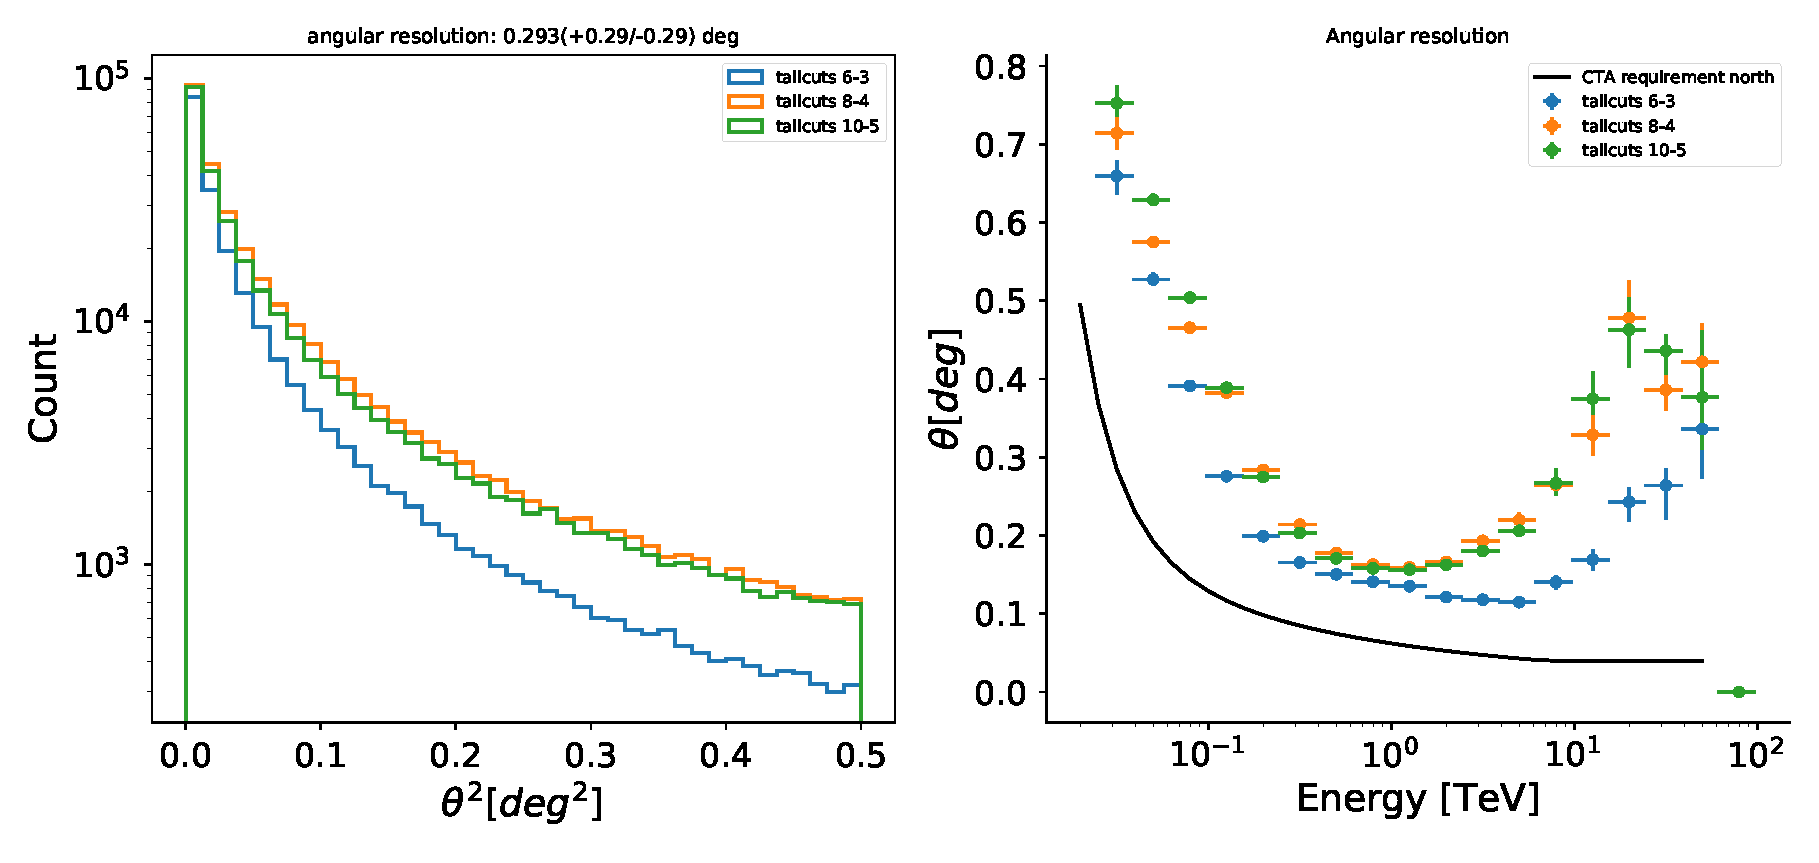
\includegraphics[width=1\textwidth]{Pictures/angular_resolution.pdf}
  \caption{\textit{Left:} $\theta^2$ plot for the \gls{mc} simulated $\gamma$ point-like events, using three sets of cleaning parameters. \textit{Right}: Angular resolution as a function of reconstructed energy.}
    \label{fig:angres}
\end{figure}

\subsubsection{$\gamma$-hadron separation}

The performance in $\gamma$-hadron separation can be studied in terms of the \gls{roc} curve of the \gls{rf} classifier. The \gls{roc} curve illustrates the diagnostic ability of a binary classifier as its discrimination threshold is varied. It is produced plotting the true positive rate(the rate of $\gamma$s correctly classified) versus the false positive rare (the rate of protons incorrectly classified as $\gamma$s) at several thresholds (gammaness). A value of 1 in true positive rate, while 0 in the false positive rate would mean a perfect classification. The closest of the \gls{roc} curve to a diagonal, the more similar to an uniformly random distribution is the classification. For this result, a subset of protons were used to test the \gls{rf} classifier together with the point-like $\gamma$s. Result is shown in figure \ref{fig:roc}. The features used for the $\gamma$/hadron classification ordered by their importance can be seen in figure \ref{fig:importances}.

\begin{figure}
\centering
 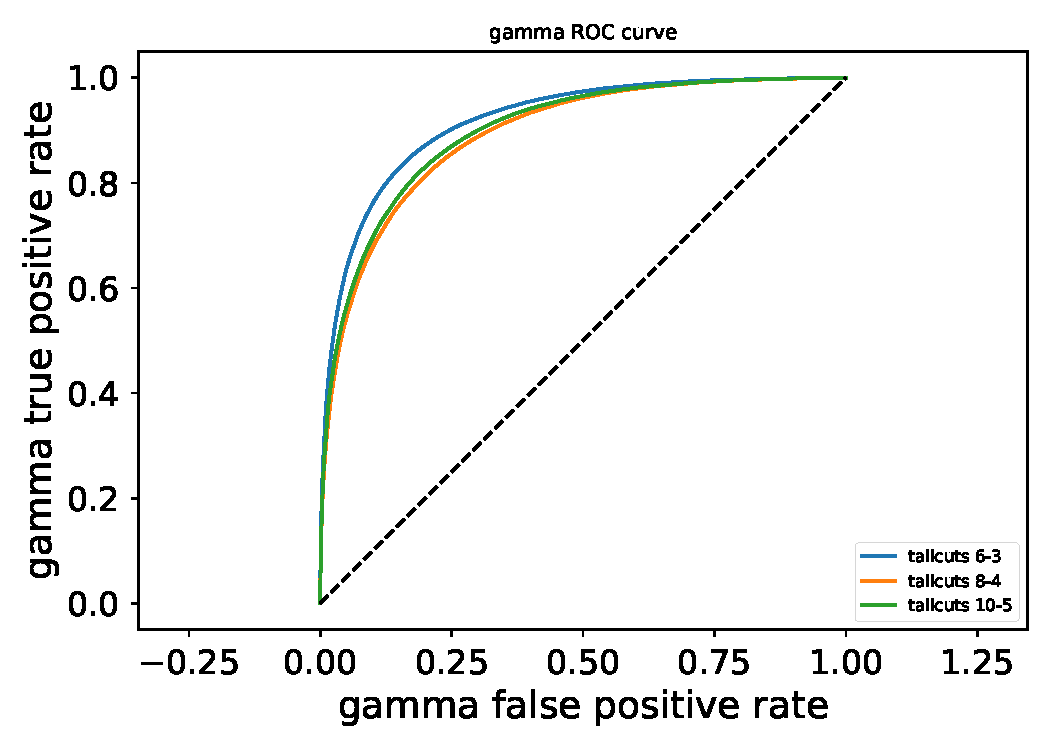
\includegraphics[width=0.6\textwidth]{Pictures/ROC.pdf}
  \caption{\gls{roc} curve of the \gls{rf} classifier applied to point-like gamma and diffuse proton events, for three different sets of cleaning parameters.}
    \label{fig:roc}
\end{figure}

\subsubsection{Effective Area}

The effective area calculated for the detection of showers from a point source with the \gls{lst}1 is shown in figure \ref{fig:effarea}.  


\begin{figure}
\centering
 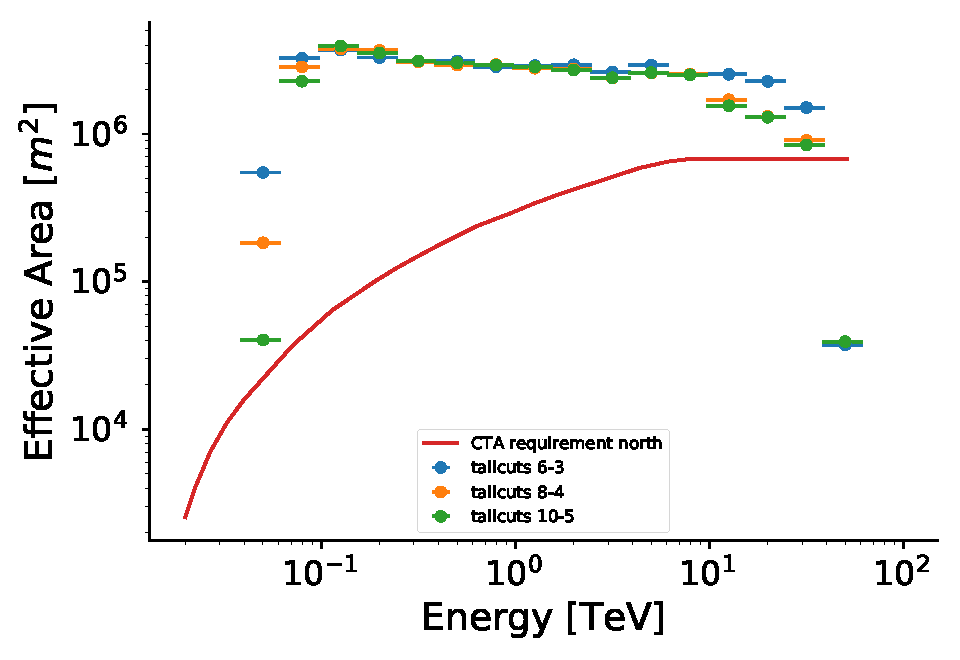
\includegraphics[width=0.6\textwidth]{Pictures/effective_area.pdf}
  \caption{Effective area per energy bin for the \gls{mc} simulated $\gamma$ point-like events, using three sets of cleaning parameters.}
    \label{fig:effarea}
\end{figure}

\subsubsection{Sensitivity}

For the calculation of the sensitivity, a subset of proton events was used as background (off) events. The point-like $\gamma$ events were used together with the protons to calculate the cuts in gammaness and $\theta^2$ which provided the best sensitivity in each of the 20 energy bins taken. To do so, the sensitivity was calculated for 10 cuts in gammaness and in $\theta^2$ for each energy. The combination of cuts giving the lower value in sensitivity, keeping a minimum of 10 $\gamma$ and proton events in the bin (both before and after re-weighting), was selected. The resulting sensitivity curve is shown in picture \ref{fig:sens}.   

\begin{figure}
\centering
 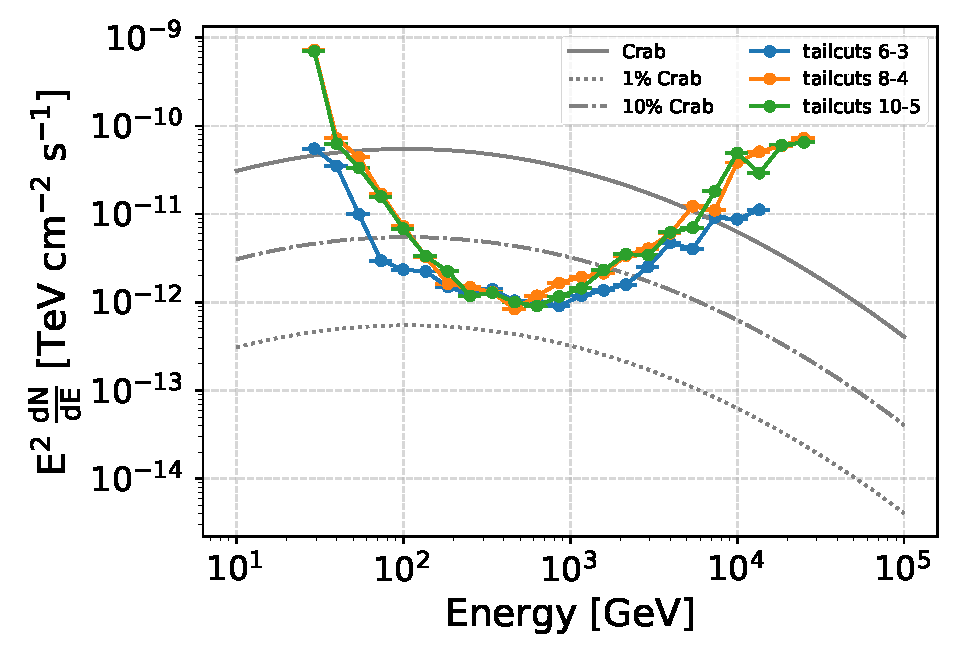
\includegraphics[width=0.8\textwidth]{Pictures/sensitivity.pdf}
  \caption{Sensitivity plot for 50h of observation of a point-like $\gamma$-ray source with a Crab-like spectrum, obtained by selecting the cuts in gammaness and $\theta2$ which provided the best differential sensitivity per energy bin. As a reference, the spectra of Crab, 10\% of Crab and 1 \% of Crab emission are shown.}
    \label{fig:sens}
\end{figure}

\section[Expectation-Maximization method for Hillas Parameters...]{Expectation-Maximization method for Hillas Parameters calculation without cleaning} \label{sec:EM}

As explained in section \ref{sec:cleanpars}, cleaning methods often require the adjust of some parameters, which have to be done empirically, trying to find a balance between a good enough background suppression without loosing too much information from the shower. The cleaning parameters affect particularly the analysis of low energy showers. In the tailcuts method, too strong cleaning thresholds tend to eliminate too many pixels of the already small low energy showers, making the task of $\gamma$-hadron separation much more difficult. Also, losing the ellipse shape of $\gamma$ showers lead to wrong calculation of Hillas parameters and consequently of the disp vector.\\
For all these reasons, with the aim to research for new analysis methods which could improve the performance of \gls{lst}, A method for image parameterization which do not require a previous cleaning has been developed. It is based in the \gls{em} algorithm, where recursively the light content in each pixel is assigned to be part of the shower or the background. In the next sections, the basic concepts of the \gls{em} method and how it can be applied to images of showers will be summarized. Then some results comparing the \gls{em} with the classic cleaning method will be shown. 

\subsection{The Expectation-Maximization algorithm}

The \gls{em} algorithm \cite{1977EM} is an iterative method for calculating maximum likelihood estimates of model parameters, where the model depends on unobserved data or latent variables. These latent variables would be those that cannot be observed in the data set, but still can influence other random variables. The algorithm will iterate until finding the model parameters and hidden variables that converge to a maximum likelihood estimation.\\
Given a statistical model which has generated a set of $X$ observed data points, which depends on a set of latent variables $Z$ and unknown parameters $\theta$, the basic iteration of the \gls{em} consist on two steps:

\begin{itemize}
\item \textbf{Expectation}: Creates an expectation function $Q(\theta | \theta^{(t)})$, which is the evaluation of the log-likelihood with the current estimate of the model parameters $\theta^{(t)}$, meaning it calculates the latent variables $Z$.
  \begin{equation}
    Q(\theta | \theta^{(t)}) = E_{Z|X,\theta^(t)}
  \end{equation}
   
\item \textbf{Maximization}: Maximizes the log-likelihood function found in the previous step to find a new set of estimated parameters.
  \begin{equation}
    \theta^{(t+1)} = arg max Q(\theta | \theta^{(t)})
  \end{equation}  
\end{itemize}

A common problem that has been successfully solved by the \gls{em} algorithm is the mixture models problem, where there is a set of data which has been produced by several density distribution functions, but is impossible to know which distribution has produced each data point. This distinction between distributions would be the latent variable. This is the particular case we face with shower images. We have a distribution of light in the pixels of the camera, an we know that some photoelectrons come from Cherenkov light, and others belong to background light from the night sky. We want to know the fraction of light in each pixel which belongs to each of the distributions.\\
We assume that the Cherenkov light will follow a bi-dimensional Gaussian distribution, which will therefore produce the typical elliptical shape in the image, and the background is simply a two dimensional constant distribution. The parameters of the model will be the usual Gaussian parameters (mean and standard deviation in two dimensions) $\{x_{0}, y_{0},\sigma_{xx}, \sigma_{yy}, \sigma_{xy}\}$ and the latent variables will be the fraction of photoelectrons from the Cherenkov shower $n_{Ch}/n$ and from the background $n_{bkg}/n$ in each pixel with n total photoelectrons.\\
The number of photoelectrons belonging to each distribution will be:

\begin{equation}
  N_{i} = \sum_{pixels} P(pixel/i)\cdot N
\end{equation}

Where $N_i$ is the number of photoelectrons produced by the distribution $i$ (Cherenkov or background), N is the total number of photoelectrons in the image and $P(pixel/i)$ is the probability of a photoelectron in the pixel to have been produced by the distribution $i$.\\
Using the Bayes theorem:
\begin{equation}\label{eq:bayes}
  P(pixel/i) = \frac{P_i(pixel) \cdot P_i}{P(pixel)}
\end{equation}
Where $P_i(pixel)$ is the probability of a photoelectron produced by the distribution $i$ to fall in the pixel, $P_i$ is the probability of a photoelectron to be produced by the distribution $i$ and $P(pixel)$ is the probability of a photoelectron to fall in the pixel. This last probability will actually be:
\begin{equation}
P(pixel) = \sum_{i} P_i \cdot P_i(pixel)
\end{equation}
Where probabilities $P_i=(P_{Ch}, P_{Bkg})$ are equal to the fraction of photoelectrons in the image belonging to the shower(background) with respect to the total number of photoelectrons. The probabilities $P_i(pixel)$ can be written as:
\begin{equation}
  \begin{split}
  & P_{Ch}(pixel) = BiGaus(x_{0}, y_{0},\sigma_{xx}, \sigma_{yy}, \sigma_{xy}) \cdot A_{pixel}\\
  & P_{bkg}(pixel) = A_{pixel}/A_{total}
  \end{split}
\end{equation}
Where $A_{pixel}$ is the area of the pixel and $A_{total}$ the sum of the areas of all pixels.\\
The loop in the \gls{em} to solve this problem will go as follows:
\begin{enumerate}
  \item An initial assumption of the Gaussian parameters is made. Because the bi-dimensional Gaussian corresponds to the Hillas ellipse, the means of the distribution will coincide with the center of gravity of the ellipse, which will be close to the pixel with higher charge. To avoid committing a mistake choosing the initial value due to an outlier pixel, we take the initial means of the Gaussian ($x_0$, $y_0$) as the coordinates of the baricenter of the three more luminous pixels. The initial values of the standard deviations are set to arbitrary high values $\sigma_{xx}=20000$, $\sigma_{yy}=20000$, $\sigma_{xy}=0$. Also we assume an initial estimation of the fraction of the light belonging to the shower and background as 50\% of the total number of photoelectrons for each.

  \item Expectation: Using the previous estimation of Gaussian parameters and fractions of photoelectrons, equation \ref{eq:bayes} is solved and the distributions of the shower and the background are obtained. For each pixel the number of photoelectrons belonging to the shower and to the background is calculated.

  \item Maximization: Using the distributions from previous steps, the parameters of the bi-dimensional Gaussian corresponding to the Cherenkov light distribution are calculated, and also the fraction of the total photoelectrons produced by each distribution (which is simply the sum of all shower and background pixels content respectively). The new Gaussian parameters will be:

    \begin{equation}
      \begin{split}
        & mean_{x} = \frac{1}{N}\sum_{pixels} n_{Ch} x_{pix}\\
        & mean_{y} = \frac{1}{N}\sum_{pixels} n_{Ch} y_{pix}\\
        & \sigma_{xx} = \frac{1}{N}\sum_{pixels} n_{Ch} x_{pix}^{2} - mean_{x}^2\\
        & \sigma_{yy} = \frac{1}{N}\sum_{pixels} n_{Ch} y_{pix}^{2} - mean_{y}^2\\
        & \sigma_{xy} = \frac{1}{N}\sum_{pixels} n_{Ch} x_{pix}^{2} y_{pix}^{2} - mean_{x}mean_{y}\\
      \end{split}
    \end{equation}
  \item Steps 2 and 3 are repeated until convergence.\\
    
\end{enumerate}

The \gls{em} method was used to calculate the Hillas parameters of a small subset of the \gls{mc} production described in section \ref{sec:mcdata} ($\sim$ 20k events of diffuse $\gamma$s and protons for training the \gls{rf}s, and $\sim$ 200k events of point-like gammas for testing the results). These parameters were used to do the energy and direction reconstruction and the $\gamma$-hadron classification. The results, compared to the ones obtained using the tailcuts cleaning and parameterization method are shown in the next section.

\subsection{Comparison of \gls{em} without cleaning and tailcuts cleaning}

In this section, results on energy resolution, angular resolution and $\gamma$-hadron separation using the \gls{em} method for Hillas parameters calculation without previous cleaning are presented, compared to the results obtained applying the classic method of tailcuts cleaning for  three sets of cleaning parameters.\\
The time parameters are not included in the features for \gls{rf} training because
 the \gls{em} code developed for this work is not compatible with the function for the calculation of time parameters in \textit{ctapipe}. 

\begin{figure}
\centering
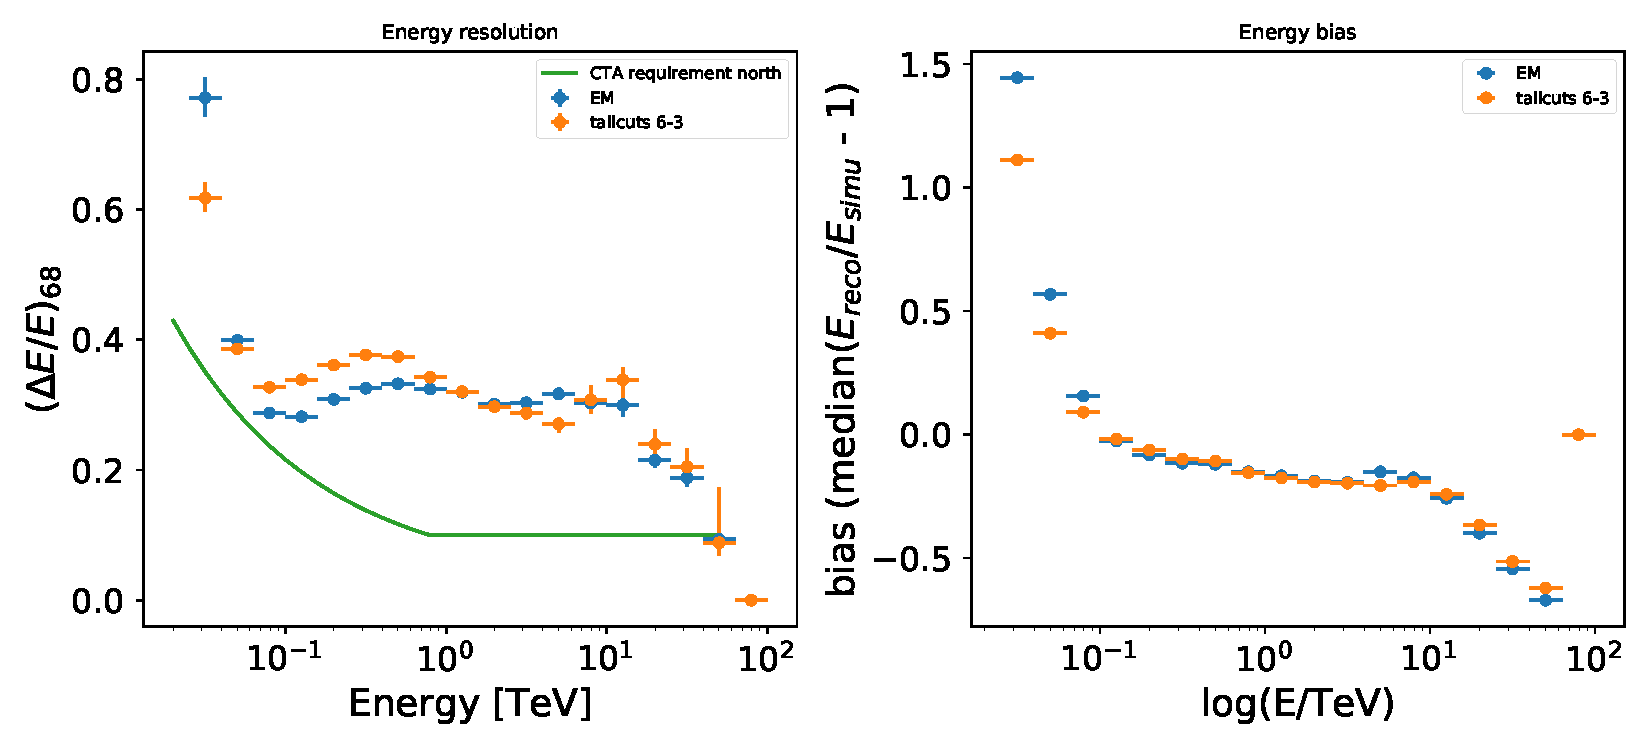
\includegraphics[width=0.8\textwidth]{Pictures/em_energy_resolution.pdf}
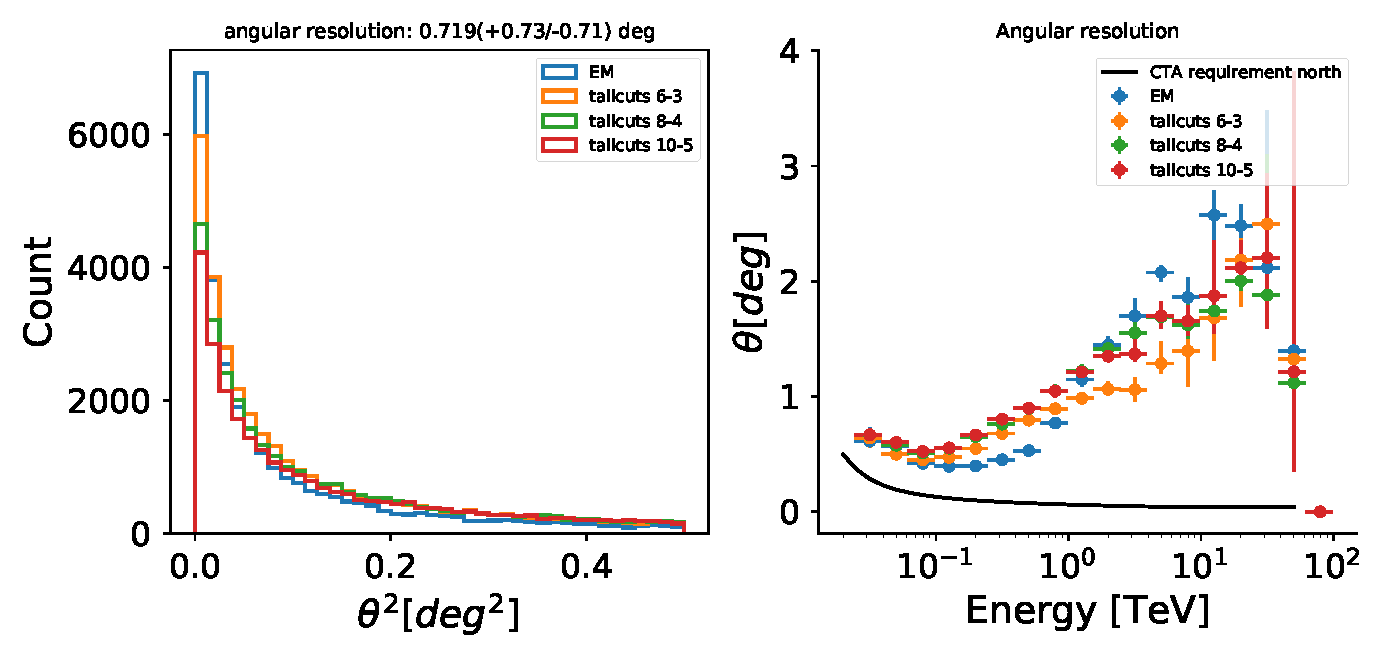
\includegraphics[width=0.8\textwidth]{Pictures/em_angular_resolution.pdf}
\minipage{0.5\textwidth}
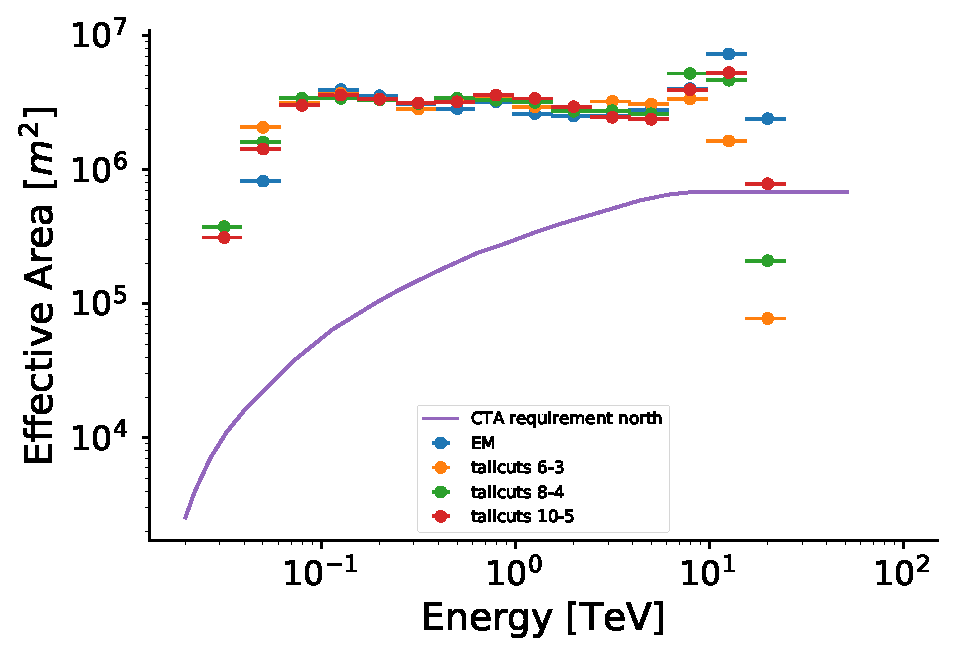
\includegraphics[width=1\textwidth]{Pictures/em_effective_area.pdf}
\endminipage
\minipage{0.5\textwidth}
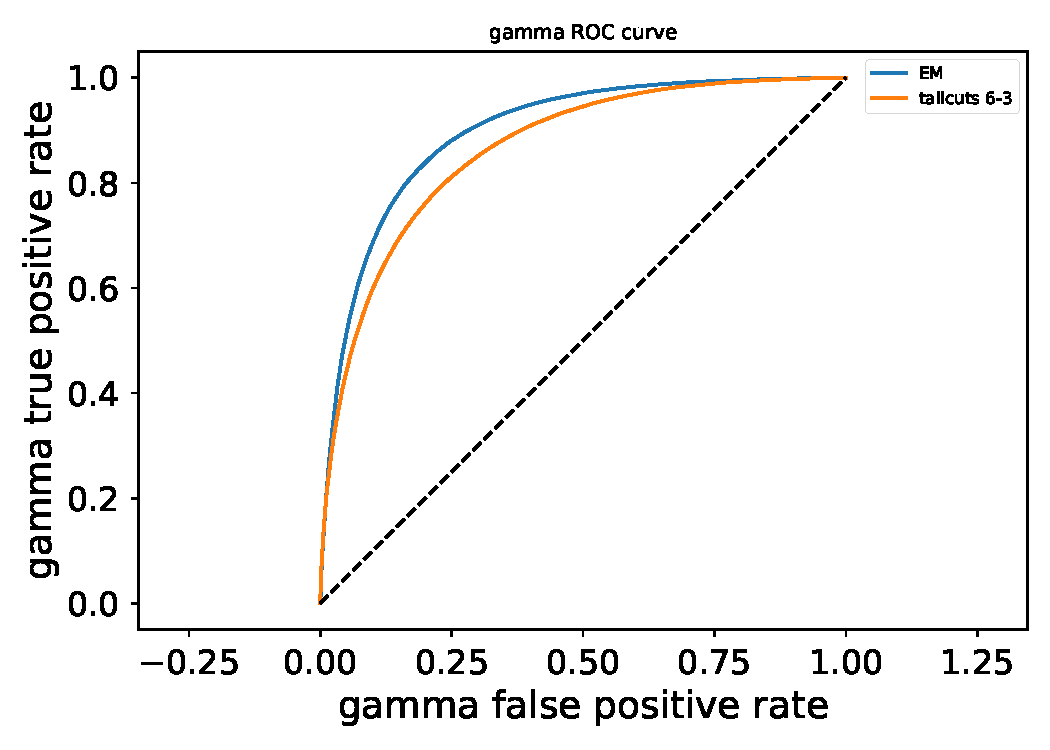
\includegraphics[width=1\textwidth]{Pictures/em_ROC.pdf}
\endminipage
  \caption{Energy resolution (\textit{top}), angular resolution (\textit{middle}), effective area (\textit{bottom-left}) and \gls{roc} curve (textit{bottom-right}) plots for a small subset of events analyzed using the \gls{em} method for Hillas parameterization without cleaning, compared to three different subsets of tailcuts cleaning parameters. }
    \label{fig:em_res}
\end{figure}

From figure \ref{fig:em_res} it can be appreciated that the results for the \gls{em} method are compatible with the tailcuts cleaning method, reassuring that this is a valid method of Hillas parameterization which allows to go through the step of cleaning which clearly can affect the performance results, as shown in section \ref{sec:performance}. The principal current caveat of the method is that it is much more time consuming than the simple tailcuts methods. Taking into account that no time optimization work has been done in the code, great improvements can be expected from the method, to become a potential useful tool for the analysis of low energy events. 

\section{Results on real data}

Since the start of the commissioning of the telescope, three datataking campaigns have been carried on, where the Crab nebula has been observed with the \gls{lst}1 during several nights, in order to test the performance of the whole instrument and the analysis tools.\\
The analysis carried on in this section has been performed over the data taken during the second Crab campaign, from January 17 to February 02 202. Telescope data is taken in runs of a certain duration, where Cherenkov events are recorded and stored in files. Each night, four kinds of runs are taken: DSR4 calibration runs (for pedestar subtraction), camera calibration runs (see section \ref{sec:calib}), data on and data off runs. Data on runs are taken pointing with the telescope to the $\gamma$-ray source, in this case the Crab nebula. Data off runs are taken pointing to a region without a $\gamma$-ray sources, where the \gls{cr} background is similar to that of the on region, allowing to estimate the background and extracting the signal events.\\
The data runs have been calibrated and parameterized using \textit{cta-lstchain} following the steps described in section \ref{sec:anachain}. The signal extractor used has been the \textit{GlobalPeakWindowSum}  and the cleaning method applied is a two level tailcuts with $Th_{high}=6$ and $T_{low}=3$. The \gls{rf} models for energy and direction reconstruction, and $\gamma$/hadron separation has been trained with \gls{mc} data, as described in sections \ref{sec:recoe} and \ref{sec:gammahsep}, and applied to the on and off data for reconstruction to DL2 data level.\\
A set of cuts, summarized in table \ref{tab:cuts}, has been applied to the data to allow a good background rejection and avoid showers with few photoelectrons or which are truncated in the edges of the camera.

\begin{table}
  \centering
    \begin{tabular}{|l|l|}
      \hline
      Intensity min & 500  \\
      Intensity max & 80000 \\
      Leakage       & < 0.2 \\
      Width/Length  & > 0.1 \\
      Gammaness     & > 0.6 \\
      \hline
      \end{tabular}
  \caption{Set of cuts applied in the prameters of the reconstructed real data from the second Crab campaign.}\label{tab:cuts}
\end{table}

The goal of the analysis performed is to calculate the significance of the source. To do so, it is necessary to calculate the number of excess events in the ON region, compared to the OFF region. In the ON region, close to the source position, an excess of events should be observed compared to the background. At further distances, the number of events should be comparable to that of the OFF region, where there are only background events. The number of background events $N_{bkg}$ in the ON region can be estimated as $N_{off}$ multiplied by a normalization factor, $n = N_{on}/N_{off}$ at a high distance from the assumed source position (the center of the camera). The significance of the excess in the ON region is defined as: 

\begin{equation}
  S = N_{ex}/\sqrt{N_{off}}
\end{equation}

Where $N_{ex}$ is defined as the Number of excess counts in the on region, calculated as $N_ex=N_{on}-N_{off} * n$. \\
The analysis can be performed following two different definitions for the distance from the source position. The first kind of analysis is the $\theta^2$ analysis, where the $\theta^2$ angle is defined as:

\begin{equation}
  \theta^2 = X_{S}^2 + Y_{S}^2 
\end{equation}

$X_{S}$ and $Y_{S}$ represent the reconstructed position of the source in camera coordinates. If the telescope is pointing to the source position, the closer of $\theta^2$ to 0 (the center of the camera), the closer to the true source position has been reconstructed the event. We can assume that background events have reconstructed source positions distributed randomly over the \gls{fov}, but the events of the source will have reconstructed positions with $\theta^2$ closer to 0. The normalization factor $n$ between the number of background events in the ON and OFF regions is calculated using events with $\theta^2$ > 0.5º. To calculate the number of excess counts and the significance, a cut in $\theta^2$ < 0.25º is applied. In picture ??, the value of $\theta^2$ is plotted for the ON and OFF regions, observing clearly an excess around $theta^2=0$. The rate of $\gamma$ events (number of events per second) can be calculated dividing the number of excess events $N_{ex}$ by the total observation time.\\

The second type of analysis is made with respect to the alpha angle, which is defined as:

\begin{equation}
  \alpha = arc cos\left(\frac{X_{c.o.g.}cos(\psi) + Y_{c.o.g.} sin(\psi)}{X_{c.o.g.}^2 + Y_{c.o.g.}^2}\right)
\end{equation}

Where $X_{c.o.g.}$ and $Y_{c.o.g.}$ are the coordinates of the center of gravity of the Hillas ellipse of the shower image, and angle $\psi$ is the angle between the semimajor axis of the ellipse and the line between the center of the camera and the center of gravity of the ellipse. The alpha angle indicate how deviated is the hillas ellipse from pointing towards the center of the camera. Events with high alpha angle are more likely to be background events, whereas $\gamma$ events will point towards the same position, close to the center, having small alpha angles. To estimate the background normalization factor $n$, events with $\alpha$ angle between 20º and 80º are used. To calculate the excess signal and sensitivity a cut in $\alpha < 8º$ is applied.\\

The $\theta^2$ and $\alpha$ plots are shown in picture \ref{fig:crabana} for the full campaign and for just one day of observation. The data was taken between January 15th and February 2nd, summing a total of 12.8 hours of observation, which combined lead to a final detection significance of 46.9 $\sigma$ for the $\theta^2$ analysis, and 21.26$\sigma$ for the $\alpha$ analysis, after applying the cuts listed in table \ref{tab:cuts}. 

\begin{figure}
  \centering
  \minipage{0.5\textwidth}
  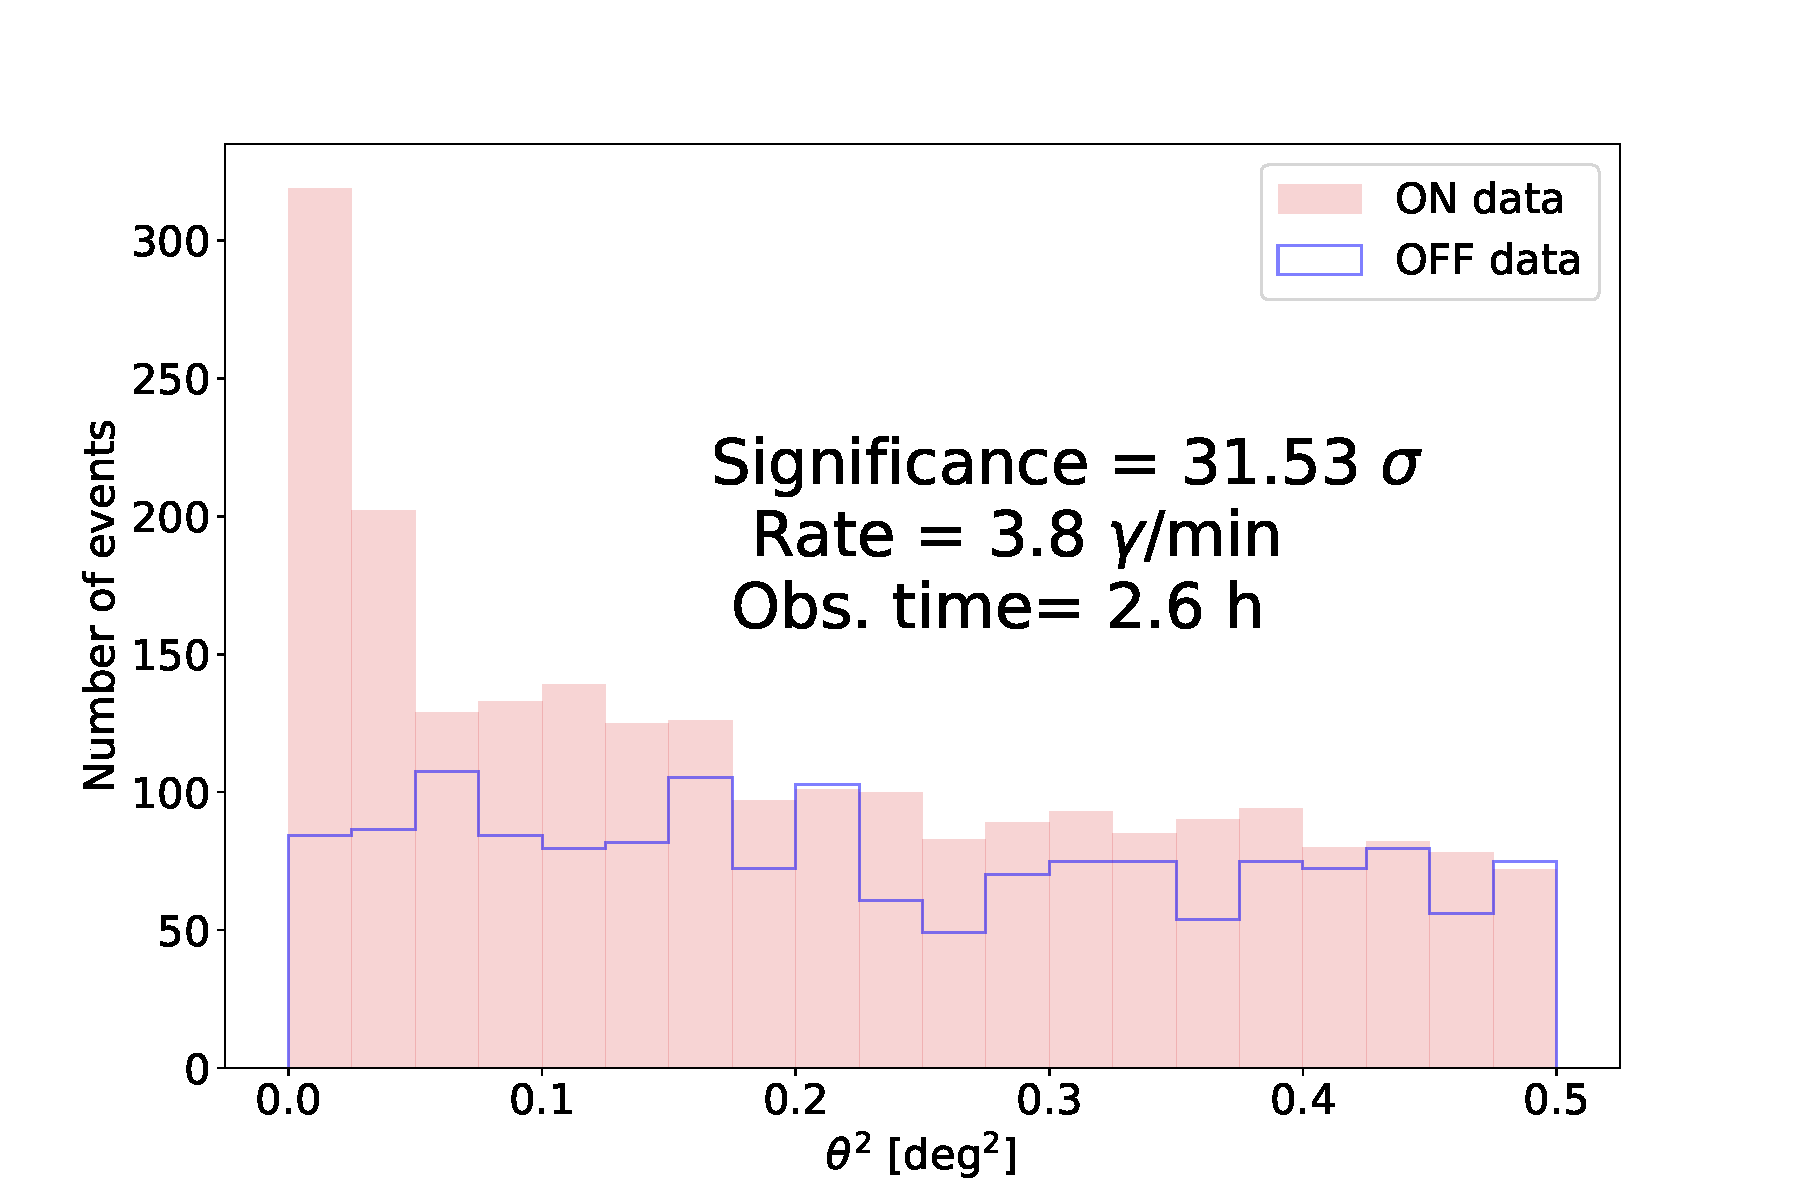
\includegraphics[width=1\textwidth]{Pictures/thetaplot_20200118_int500_gammaness0-600000.pdf}
  \endminipage
  \minipage{0.5\textwidth}
  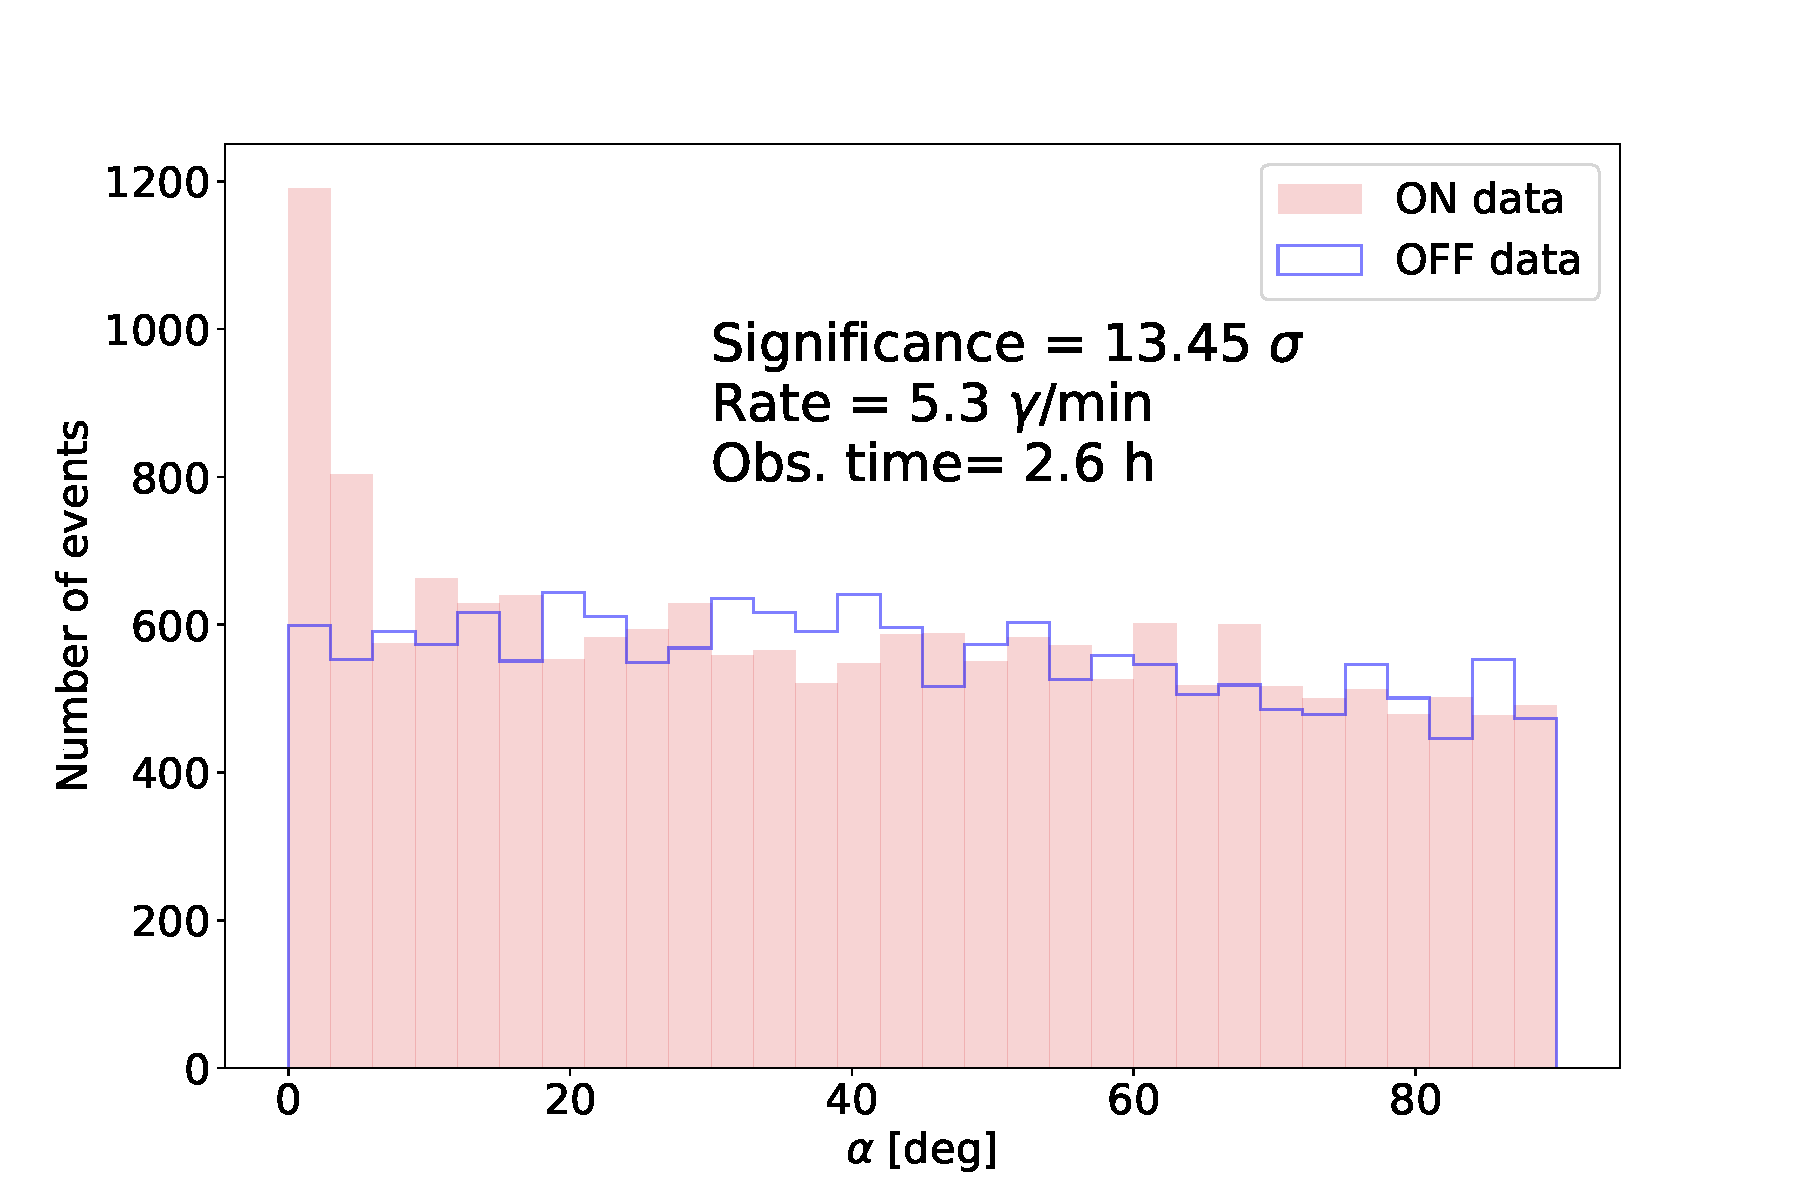
\includegraphics[width=1\textwidth]{Pictures/alphaplot_20200118_int500_gammaness0-600000.pdf}
  \endminipage \\
  \minipage{0.5\textwidth}
  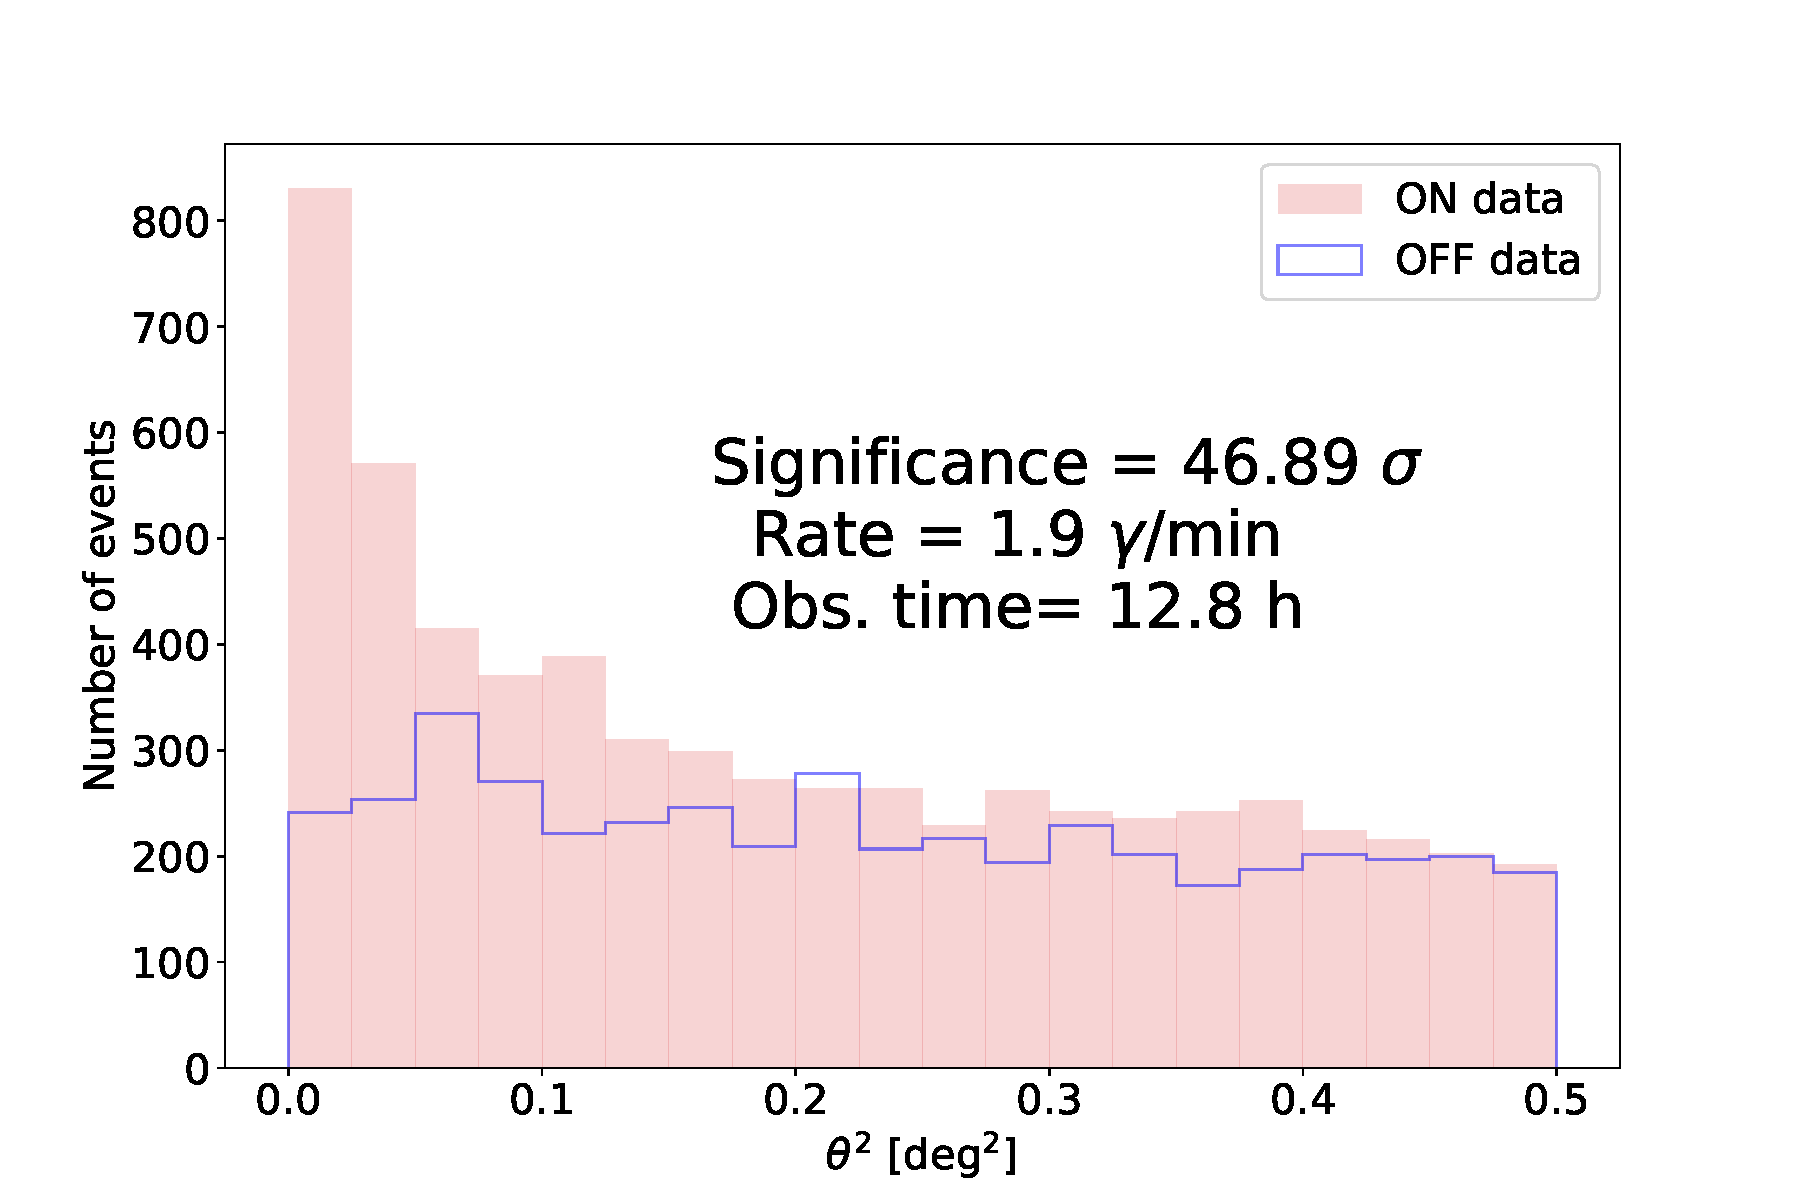
\includegraphics[width=1\textwidth]{Pictures/thetaplot_int500_gammaness0-6.pdf}
  \endminipage
  \minipage{0.5\textwidth}
  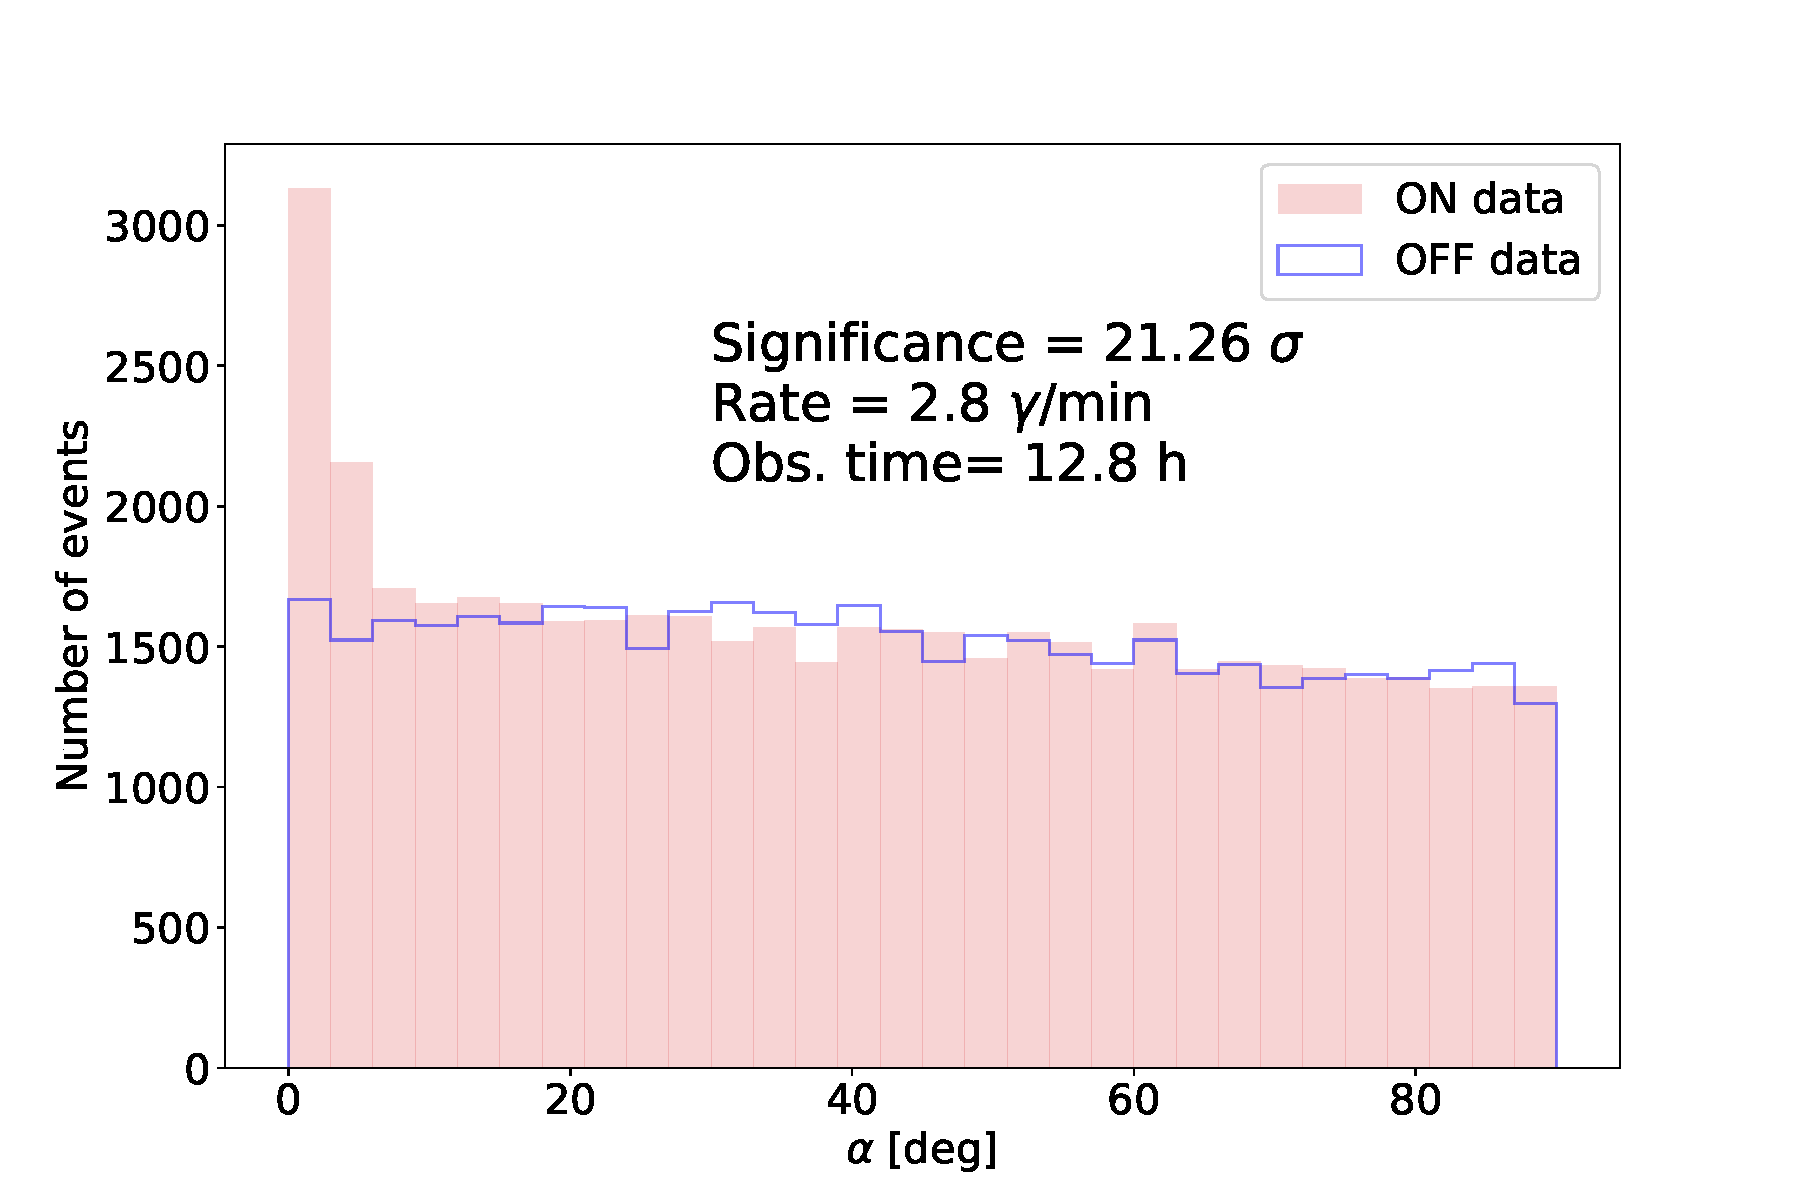
\includegraphics[width=1\textwidth]{Pictures/alphaplot_int500_gammaness0-6.pdf}
  \endminipage \\
  \caption{\textit{Top}: $\theta^2$ (\textit{left}) and $\alpha$ (\textit{right}) plots for the Crab data taken during the night of the 18/01/2020. \textit{Bottom}: $\theta^2$ (\textit{left}) and $\alpha$ (\textit{right}) plots for the data taken during full second Crab campaign, from 15/01/2020 to 02/02/2020. Results are calculated after applying the cuts from table \ref{tab:cuts}.} \label{fig:crabana}
\end{figure}

\section{Summary and conclusion}

Along this chapter, the chain for the single telescope data analysis of \gls{lst}1 has been described, and successfully used to derive the performance of the \gls{lst}1, and to analyze the first real data taken with the instrument.\\
About the performance estimated using \gls{mc} simulations, it has been shown that the energy resolution reaches an error as low as 20\% in the range from $\sim 100$ GeV to a few TeV and the angular resolution in the same energy range is $\sim 0.2$º. From the three sets for tailcuts parameters, the one giving best results has been the 6-3 tailcuts. The best sensitivity of \gls{lst}1 for 50 hours of observation is reached in the range between 100 GeV and 1 TeV, going below the 10\% of the Crab flux.\\
The \gls{em} method for Hillas parameterization without cleaning has been presented as a potential alternative, with similar performance to the classic tailcuts cleaning (without time parameters), to avoid the necessity to adjust the tailcuts parameters which clearly affect the performance results. This method is useful for low energy events, with very few photoelectrons, where tailcuts cleaning can suppose the loss of information from the shower.  

\end{document}
